\documentclass[12pt]{report}
%\usepackage[a4paper, total={15cm, 20cm}]{geometry}

\usepackage{amsmath}
\usepackage{amsthm}
\usepackage{amssymb}
\usepackage{amsbsy}
\usepackage{graphicx}
\usepackage{natbib}
\usepackage{url}
\usepackage{subcaption}
\usepackage[nottoc]{tocbibind}
\usepackage{hyperref}

\DeclareMathOperator{\expfamily}{ExpFamily}
\DeclareMathOperator{\expectation}{\mathbb{E}}
\DeclareMathOperator{\variance}{\mathbb{V}ar}
\DeclareMathOperator{\cov}{\mathbb{C}ov}
\DeclareMathOperator{\corr}{\mathbb{C}orr}
\DeclareMathOperator{\bernoulli}{Bernoulli}
\DeclareMathOperator{\betaDist}{Beta}
\DeclareMathOperator{\dirichlet}{Dir}
\DeclareMathOperator{\bin}{Bin}
\DeclareMathOperator{\MN}{Multinomial}
\DeclareMathOperator{\prob}{\mathbb{P}}
\DeclareMathOperator{\trace}{Tr}
\DeclareMathOperator{\normal}{N}
\DeclareMathOperator{\gammaDist}{Gamma}
\DeclareMathOperator{\poisson}{Poisson}

\newcommand{\RSS}{\mathrm{RSS}}
\newcommand{\euler}{\mathrm{e}}
\newcommand{\diff}{\mathrm{d}}
\newcommand{\T}{^\textup{T}}
\newcommand{\dotdotdot}{_{\phantom{.}\cdots}}
\newcommand{\BIC}{\textup{BIC}}

\newcommand{\vect}[1]{\mathbf{#1}}
\newcommand{\vectGreek}[1]{\boldsymbol{#1}}
\newcommand{\matr}[1]{\mathsf{#1}}

\newtheorem{theorem}{Theorem}
\newtheorem{algorithm}{Algorithm}


\begin{document}

%=====TITLE PAGE======
\begin{titlepage}
\centering
\vspace*{1cm}
        
        \LARGE
        \textbf{Inside-Out: Characterisation of Computed Tomography Noise in Projection and Image Space with Applications to 3D Printing}
        
		\large        
        
        \vspace{2cm}
        {OxWaSP 2015-16 University of Warwick Cohort}
        
        \vspace{1cm}
        {Mini-Project 1 Report}
        
        \vspace{1cm}
        {Sherman Ip}

        \vspace{1cm}
        {Supervisor: Dr.~J.~Brettschneider (Statistics, Warwick)}
        
        \vspace{1cm}
        {Supervisor: Prof.~T.~Nichols (Statistics, Warwick)}
        
        \vspace{1cm}
        {10th June 2016}
\end{titlepage}

%======ABSTRACT=========
\begin{abstract}
X-ray computed tomography can be used to do quality control on 3D printed samples. However there are sources of error in the 3D printing, how the photons behave and in the X-ray detector. This project aims to find a relationship between the mean and variance of the grey values of each pixel in images obtained from the X-ray detector by fitting linear regressions. In addition, latent variable models such as principle component analysis, factor analysis and the compound Poisson were attempted to be fitted to find sources of variance.
\end{abstract}

%======ACKNOWLEDGEMENT=========
\renewcommand{\abstractname}{Acknowledgements}
\begin{abstract}
\begin{itemize}
	\item Supervisors: Julia Brettschneider and Tom Nichols
	\item Inside Out Team: Wilfrid Kendall, Audrey Kueh, Jay Warnett and Clair Barnes
	\item OxWaSP 2015 Cohort: Nathan Cunningham, Giuseppe di Benedetto, Beniamino Hadj-Amar, Jack Jewson, Ella Kaye, Leon Law, Kaspar Martens, Marcin Mider, Xenia Miscouridou, Paul Vanetti and Andi Wang.
	\item EPSRC Funding: EP/L016710/1
\end{itemize}
\end{abstract}

%=====FRONT MATTER=====
\tableofcontents
%\listoffigures
%\listoftables

%======INTRODUCTION========
\chapter{Introduction}

3D printing, formally additive manufacturing \cite{wong2012review}, has recently became state of the art technology which manufactures objects of complicated shapes with very high precision. It was developed in the 1980's \cite{kodama1981automatic} but recently it has been commercialised and is used in medical science \cite{kang20163d} and engineering \cite{wong2012review}. Because of such a wide range of applications, there has been a need for quality control and this can be done by scanning the 3D printed sample using X-ray computed tomography.

The Inside-Out group at the University of Warwick aims to develop statistical methodology for using computed tomography scans to do quality control on 3D printed samples. Recent research include how the penumbra can be modelled \cite{kueh2014modelling}, simulating and detecting defects and on the behaviour of dead pixels \cite{brettschneider2014spatial}.

The aim of this specific project was to do linear regression on the mean and variance of the grey values in the computed tomography images to find explanatory relationships. Separately, latent variable models were fitted to the images to find sources of variance. Latent variable models include principle component analysis, factor analysis and compound Poisson.

This report was written in a Master dissertation style and assumes knowledge up to graduate level in physics and statistics. The mathematics and statistics used can be reviewed in undergraduate textbooks \cite{riley2006mathematical} \cite{rice2009mathematical}, however complicated matrix calculus results will be stated without proof in Appendix \ref{chapter:matrixCalculus}.

%======LITERATURE REVIEW========
\chapter{Literature Review}
Computed tomography (CT) scanning is a 3D imaging technique. It does this by reconstructing the geometry of the sample through a series of 2D X-ray images of the sample. The sample rotates after each image taken \cite{cantatore2011introduction}.

Figure \ref{fig:x_ray_ct} shows a diagram on how CT scanning works. A 2D image is taken by projecting X-ray photons onto the stationary sample. The photons are then scattered or absobred by the sample.  Some of these photons are then detected by an X-ray detector on the other side of the sample, which produces an image. After an image has been taken, the object rotates and another image is taken. Finally after a number of images, a 3D reconstruction of the object can be estimated \cite{cantatore2011introduction}.

\begin{figure}
\centering
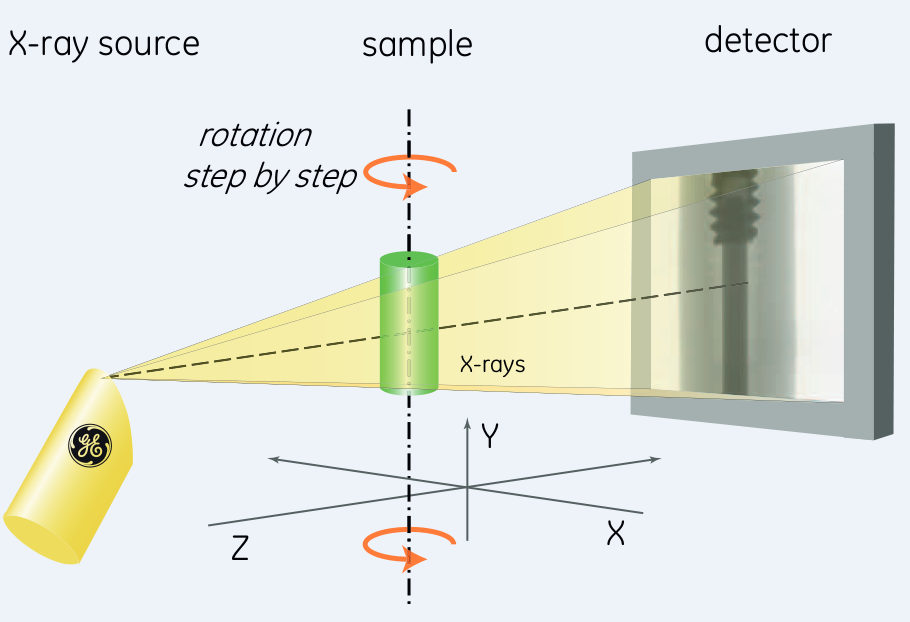
\includegraphics[width=0.7\textwidth]{figures/x_ray_ct.png}
\caption{X-ray computed tomography reconstructs the sample by projecting photons onto a rotating sample. The photons are then detected by the detector. \emph{Source: http://www.phoenix-xray.com/}}
\label{fig:x_ray_ct}
\end{figure}

CT scanning was invented by G. Hounsfield \cite{hounsfield1980computed} in the 1980's and it was mainly used for medical imaging. The setup for CT scanning is different when scanning patients because the detector and X-ray source rotates around the patient \cite{cantatore2011introduction}. Recently CT has been used industrially for non-destructive testing in manufacturing \cite{cantatore2011introduction}. One possible application would be inspecting 3D printed samples.

There are many sources of error in CT scanning \cite{cantatore2011introduction} and this can cause problems when reconstructing the geometry of the sample. Sources of error include: defects in the detector, environmental noise and the behaviour of photons.

This chapter aims to give brief description on how CT scanning works.

\section{X-Ray Production}
Photons in CT scanning are produced in an X-ray tube. In an X-ray tube, a cathode, consisting of a heated filament, fires projectile electrons through an electric potential to a target which forms the anode \cite{michael2001x}, as shown in Figure \ref{fig:x_ray_tube}. Most of the kinetic energy of the projectile electrons is converted into heat however some is converted into electromagnetic radiation. This depends on how the projectile electrons interact with the atoms in the anode \cite{cantatore2011introduction}.

\begin{figure}
\centering
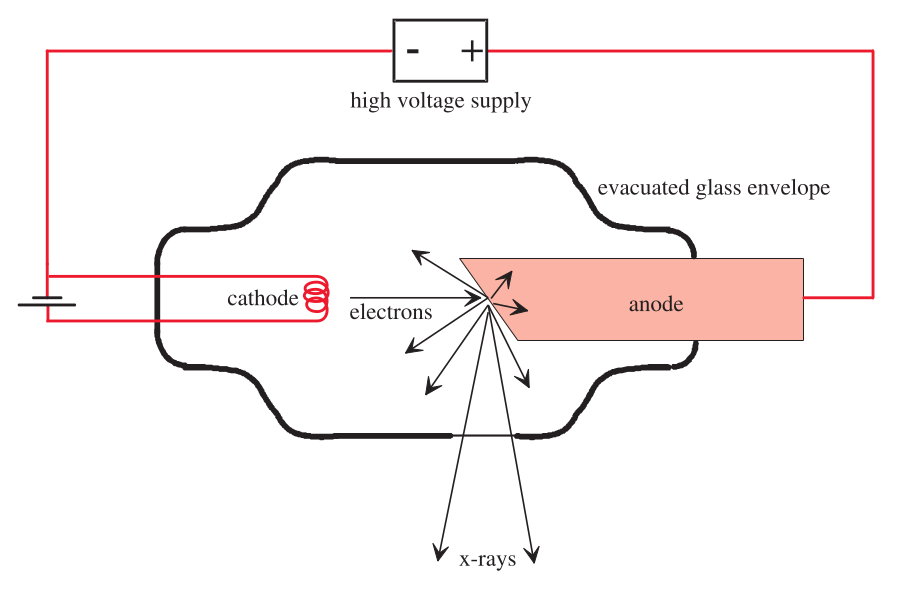
\includegraphics[width=0.8\textwidth]{figures/x_ray_tube.png}
\caption{An X-ray tube produces photons by firing projectile electrons from a cathode to an anode. \emph{Source: G.~Michael (2001) \cite{michael2001x}}}
\label{fig:x_ray_tube}
\end{figure}

Bremsstrahlung radiation is the result of projectile electrons deaccelerating due to the electrostatic field produced by nucleus of the target. The kinetic energy of the projectile electrons is then converted to electromagnetic radiation to produce X-ray radiation. As a result, the photon energies in bremsstrahlung radiation is  a continuous spectrum and can range up to the maximum kinetic energy of the projectile electrons \cite{michael2001x}.

Characteristic radiation is due to projectile electrons colliding with electrons in the target atom and ionizing them. This produce vacancies in the electron shell and emits photons when the electrons in the target atom drops down back to the ground state. The energy of the emitted radiation is monoenergetic and depends on the binding energy of the target's atoms \cite{michael2001x}.

A typical energy spectrum of photons emitted from an X-ray tube is as shown in Figure \ref{fig:x_ray_spectrum}. The energy spectrum consist of both bremsstrahlung and characteristic radiation \cite{michael2001x}.

\begin{figure}
\centering
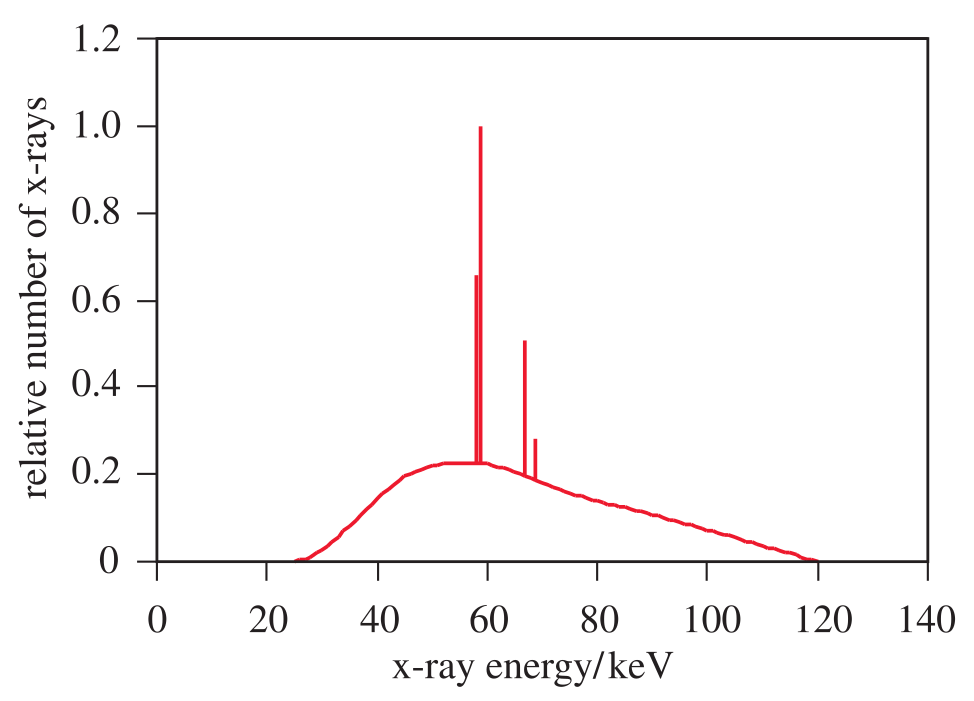
\includegraphics[width=0.8\textwidth]{figures/x_ray_spectrum.png}
\caption{A typical energy spectrum of photons emitted from an X-ray tube. The continuous spectrum is the result of Bremmsstrahlung radiation. The peaks are the result of characteristic radiation. \emph{Source: G.~Michael (2001) \cite{michael2001x}}}
\label{fig:x_ray_spectrum}
\end{figure}

The voltage and current can be varied in the X-ray tube to produce different energy spectrums and rate of photon production. This can vary the results produced when collecting CT data \cite{cantatore2011introduction}. Another important factor is the focal spot size because smaller spot sizes produce sharper edges. Larger spot sizes produce unsharp results and this is know as the penumbra effect, as shown in Figure \ref{fig:x_ray_penumbra}. However spot sizes too small can produce concentrated heat \cite{welkenhuyzen2009industrial} and can damage the X-ray tube.

\begin{figure}
\centering
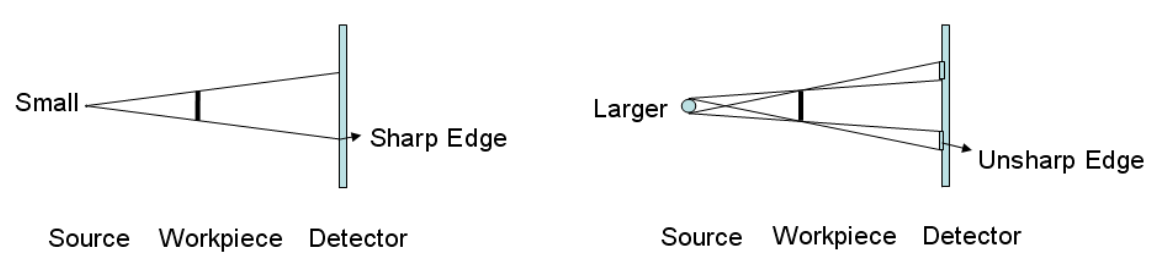
\includegraphics[width=1\textwidth]{figures/x_ray_penumbra.png}
\caption{Larger focal spot sizes produces unsharp results. This is know as the penumbra effect. \emph{Source: F.~Welkenhuyzen et al.~(2009)\cite{welkenhuyzen2009industrial}}}
\label{fig:x_ray_penumbra}
\end{figure}

\section{X-Ray Interactions}
Photons emitted by the X-ray tube are projected onto the sample and interacts with it in a number of ways \cite{cantatore2011introduction}.

The sample can effectively absorb photons via the photoelectric effect or pair production \cite{cantatore2011introduction}. In the photoelectric effect, the photons transfers all its energy to a bounded electron and ejects it from the atom \cite{millikan1916direct}. In pair production, the photons convert into electron-position pairs by interacting with the Coulomb field of the sample's atomic nucleus \cite{hubbell2006electron}. In addition to getting absorbed, photons can be scattered by the sample. This happens when photons collide inelastically with and transfers its energy to the sample's electrons. This process is know as Compton scattering \cite{compton1923quantum}.

Suppose a mono-energetic X-ray pencil beam attenuating through an object with varying attenuation coefficient in position $\mu=\mu(x)$. The beam starts at $x=0$ and is detected at $x=L$, then the attenuation (decrease in X-ray intensity from $I_0$ to $I_1$) is given as \cite{cantatore2011introduction}
\begin{equation}
I_1 = I_0\exp\left[\int_0^L-\mu(x)\diff x\right].
\label{eq:beerLaw}
\end{equation}
By comparing the intensity before and after attenuation, the integral of the attenuation coefficient along the path of the X-ray can be calculated. Because of the discrete nature of pixels, the integral is usually replaced by a sum \cite{michael2001x}. 

However it was shown that the attenuation coefficient does depend on the energy of the photons \cite{elbakri2002statistical}. Thus $\mu=\mu(x,E)$ should be made dependent on the energy of the photons \cite{cantatore2011introduction}. In general low energy photons are more likely to be absorbed than high energy photons, this increases the average energy of the attenuated photons and can be a source of error in CT scanning. This is referred to beam hardening and can cause inaccuracies in Equation \eqref{eq:beerLaw} \cite{michael2001x}. This can be reduced by placing a thin sheet of filter to absorb low energy photons \cite{welkenhuyzen2009industrial} or by correcting it in the data analysis stage \cite{michael2001x}.

\section{Detection and Reconstruction}
Most X-ray detectors are scintillator-photodiode detectors. The photons interact with the scintiallator material and produces visible light. The visible light is then detected by photodiodes and coverts it into electricical current \cite{michael2001x}. The detectors used in CT scanning are flat bed scanner which consist of an array of panels of photodiodes \cite{cantatore2011introduction}.

The scale of the 2D images can be calibrated with the use of reference standards \cite{bartscher2007enhancement}. The methods used to reconstruct the 3D geometry of the sample is called the filtered back-projection \cite{michael2001x}. The mathematics can be reviewed in \cite{brooks1976principles} and recent methods consider  polyenergetic photons \cite{elbakri2002statistical}.

%======ABOUT THE DATA========

\chapter{About the Data}\label{chapter:about_the_data}

A dataset was given for this project. 100 images of a stationary cuboid, with its vertices in the middle, were taken using a Perkin Elmer XRD 1621 digital X-ray detector. These greyscale images were 1\,996$\times$1\,996 pixels in size and have a colour depth of 16 bits. This means each pixel can have grey values which take integer values from 0 to $2^{16}-1$ inclusive. In addition, these images were calibrated so that the air has grey value of 60\,000. As a result, the units of the grey values have arbitrary units. Unfortunately a scale, in terms of distance, cannot be established because no calibration was performed. A sample of the images can be viewed in Figure \ref{fig:block_montage}.

\begin{figure}[htp]
\centering
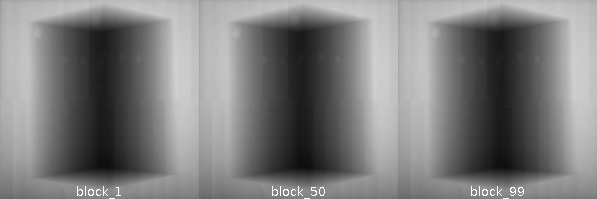
\includegraphics[width=1\textwidth]{figures/block_montage.jpg}
\caption{The 1st, 50th and 99th image in the dataset of an X-ray image of a cuboid.} 
\label{fig:block_montage}
\end{figure}

The X-ray tube was stated to have the following properties, with the number of significant figures stated as given and no error bars given:
\begin{itemize}
	\item Voltage = $V$ = 100 kV
	\item Power = $P$ = 33.0 W
	\item Exposure time = $\tau$ = 500 ms
	\item Target material is tungsten.
\end{itemize}
From this, some additional properties of the X-ray can be estimated. It is given that the efficiency of photon production $\eta$ is \cite{michael2001x}
\begin{equation}
\eta = aVZ =8.1\times10^{-3}
\end{equation}
where $a=1.1\times 10^{-1}\text{ V}^{-1}$ is a constant and $Z=74$ is the atomic number of tungsten. The rate of photon $\nu$ and energy per photon $E$ can be calculated
\begin{equation}
\nu =\frac{\eta P}{V e}=1.7\times10^{13}\text{ s}^{-1}
\end{equation}
\begin{equation}
E = Ve = 1.0\times10^{2}\text{ keV}
\end{equation}
where $e$ is the charge per electron.

\section{Histogram}
The distribution of the grey values of all the pixels in the dataset is shown in Figure \ref{fig:block_histogram}. It was observed that there were 3 distinct peaks in the histogram at grey values:
\begin{itemize}
	\item$\sim2\times10^4$ arb.~unit
	\item$\sim4\times10^4$ arb.~unit
	\item$\sim5\times10^4$ arb.~unit.
\end{itemize}
By doing a threshold, as shown in Figure \ref{fig:block_threshold}, it was clear that the main 3 sources of the grey values were the 3D printed sample, the background and the foam holder at the bottom of the image.

\begin{figure}[htp]
\centering
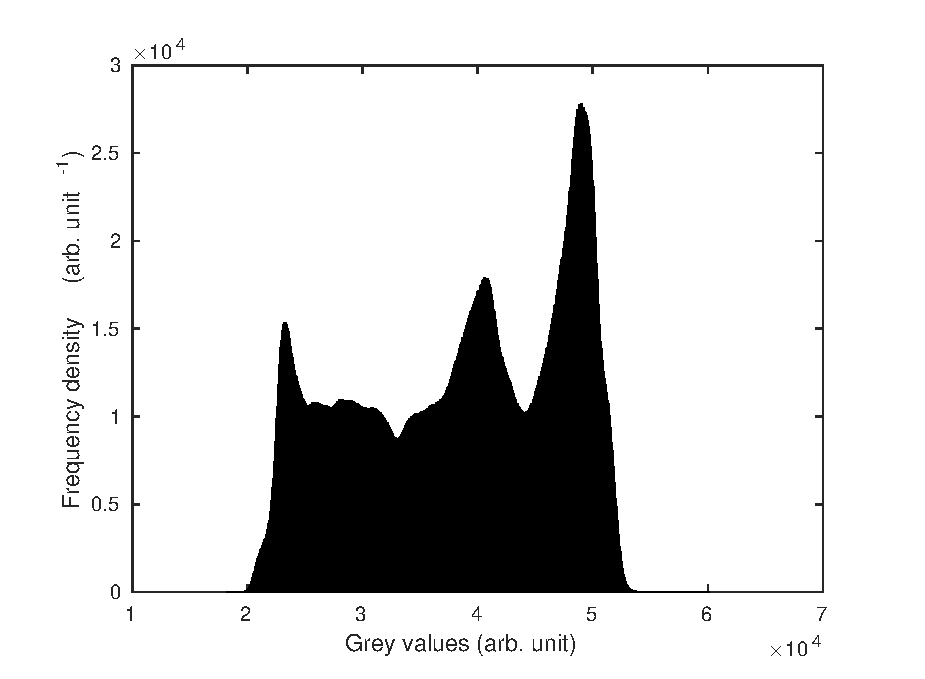
\includegraphics[width=0.75\textwidth]{figures/block_histogram.eps}
\caption{Histogram of the grey values of all the pixels in the 100 images from the dataset. The grey values ranged from 18\,286 to 60\,045.}
\label{fig:block_histogram}
\end{figure}

\begin{figure}[p]
	\centering
	\begin{subfigure}[b]{0.45\textwidth}
		\centering
		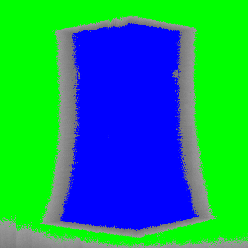
\includegraphics[width=0.8\textwidth]{figures/block_threshold.png}
		\caption{Threshold pixels}
	\end{subfigure}
	\begin{subfigure}[b]{0.45\textwidth}
		\centering
		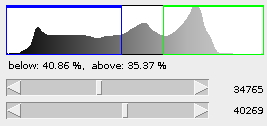
\includegraphics[width=1\textwidth]{figures/block_threshold_histogram.png}
		\caption{Histogram}	
	\end{subfigure}
	\caption{A threshold was selected to highlight pixels with certain grey values. Blue: Pixels with grey values less than 34\,765. Green: Pixels grey values more than 40\,269.}
	\label{fig:block_threshold}
\end{figure}

\section{Normality}

For a given pixel, a Normal distribution was fitted on the 100 grey values and the $\chi^2$ goodness of fit test was conducted. This was done on all $1\,996^2$ pixels as shown in Figure \ref{fig:initial_fit_normal_test}. When considering the Bonferoni correction \cite{weisstein2004bonferroni} for multiple hypothesis testing, the Normal distribution appeared to be a good fit because only 9 pixels have $p$ values less than 10\%. In addition, these significant pixels did not seem to cluster and appear random in space. When ignoring the Bonferoni correction, there was a suspicious patch of low $p$ values on the bottom right.

\begin{figure}[p]
\centering
	\begin{subfigure}[b]{0.75\textwidth}
		\includegraphics[width=1\textwidth]{figures/initial_p.eps}
		\caption{$p$ values}
	\end{subfigure}
	\begin{subfigure}[b]{0.75\textwidth}
		\includegraphics[width=1\textwidth]{figures/initial_p_log10.eps}
		\caption{$\log_{10} p$ values}
	\end{subfigure}
	\caption{$p$ values from the $\chi^2$ goodness of fit test on fitting the Normal distribution on the grey values for each pixel. In b) circled are pixels with $p$ values less than 10\%, corrected for multiple hypothesis testing using the Bonferroni correction.}
	\label{fig:initial_fit_normal_test}
\end{figure}

\section{Autocorrelation}
The sample mean and standard error of the grey values for each of the 100 images were taken and plotted as a time series as shown in Figure \ref{fig:timeSeries}. There was evidence of dependence between samples by looking at the sample autocorrelation plots as shown in Figure \ref{fig:timeSeries_acf_pacf}. Because there was a peak at lag 1 in the sample partial autocorrelation plot, the time series could be modelled using an autoregressive model with one parameter.

\begin{figure}[p]
	\centering
	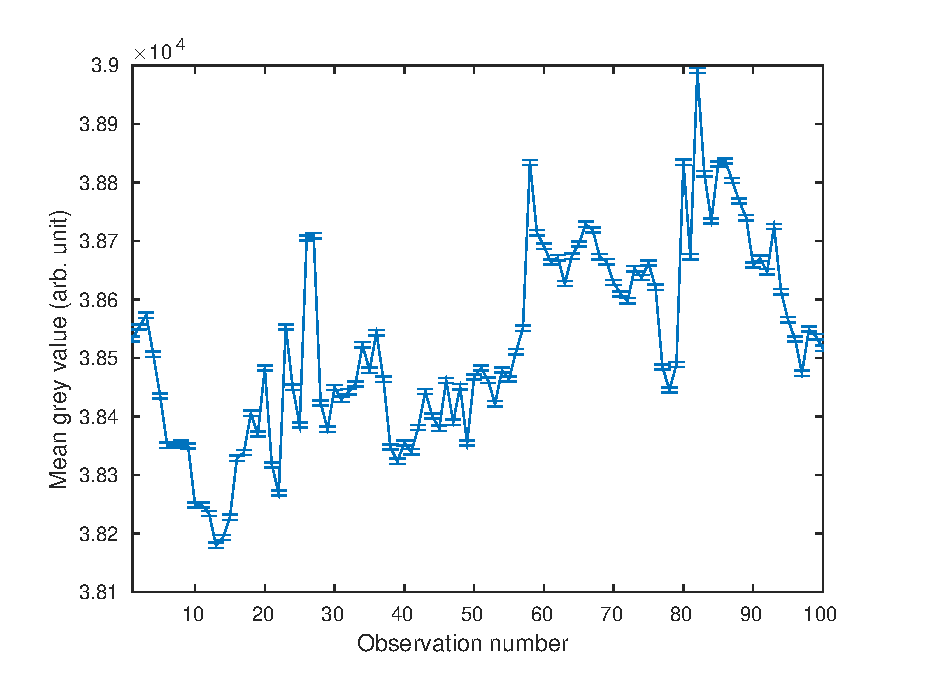
\includegraphics[width=0.75\textwidth]{figures/initial_timeSeries.eps}
	\caption{The sample mean and standard error over all the grey values for each of the 100 images.}
	\label{fig:timeSeries}
\end{figure}

\begin{figure}[p]
	\centering
	\begin{subfigure}[b]{0.45\textwidth}
		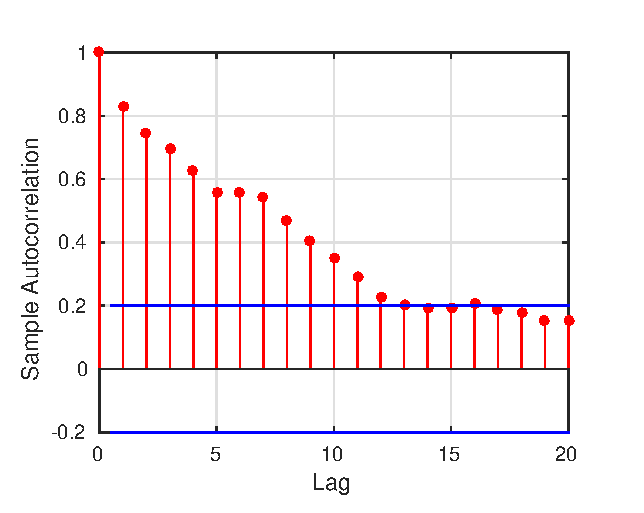
\includegraphics[width=1\textwidth]{figures/initial_acf.eps}
		\caption{Sample autocorrelation}
	\end{subfigure}
	\begin{subfigure}[b]{0.45\textwidth}
		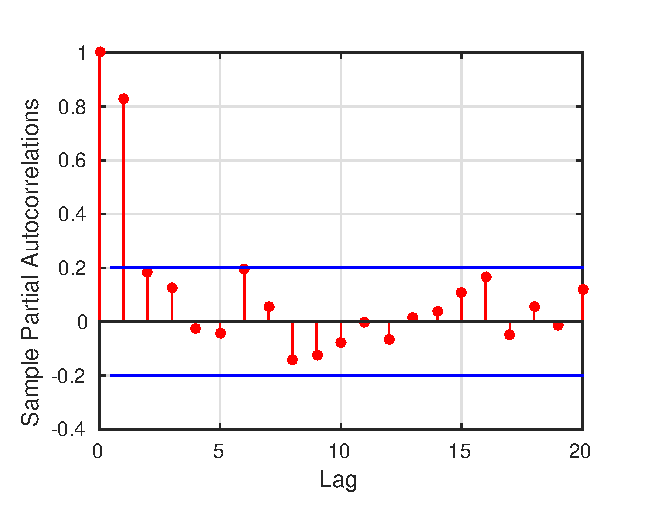
\includegraphics[width=1\textwidth]{figures/initial_pacf.eps}
		\caption{Sample partial autocorrelation}
	\end{subfigure}
	\caption{Sample autocorrelation and partial autocorrelation of the mean grey values of each image as a time series.}
	\label{fig:timeSeries_acf_pacf}
\end{figure}

%==========MEAN AND VARIANCE===========================

\chapter{Mean and Variance Relationship}

The aim of this chapter was to do supervised learning on predicting the variance of the pixel's grey values given its sample mean. This was done by fitting a linear regression to obtain a explanatory model. Once a good model was found, a single CT scan can be used to quantify the uncertainty on each pixel's grey values. This uncertainty then can be carried forward when doing volumetric reconstruction.

Figure \ref{fig:histogramHeatmap} shows the sample variance and sample mean of all the pixel's grey values. It can be seen that for sample means of $(4.5\pm0.5)\times 10^4$, the range of sample variances increased. In addition, there were a few outliers with extremely large sample variances, one example can be seen in Figure \ref{fig:scatterMeanVar}.

To take into consideration outliers, a simple weighted least squares regression was done to give less weight on outliers.

\begin{figure}
	\centering
	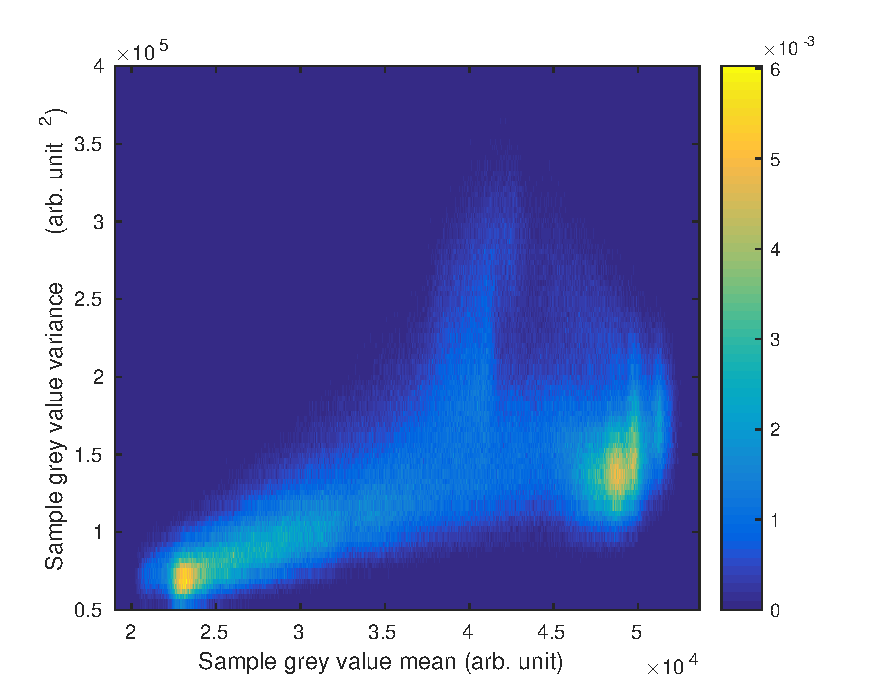
\includegraphics[width=0.75\textwidth]{figures/meanVar/histogramHeatmap.eps}
	\caption{Frequency density plot of the sample variance against sample mean of all $1\,996^2$ pixel's grey values.}
	\label{fig:histogramHeatmap}
\end{figure}

\begin{figure}
	\centering
	\begin{subfigure}[b]{0.45\textwidth}
		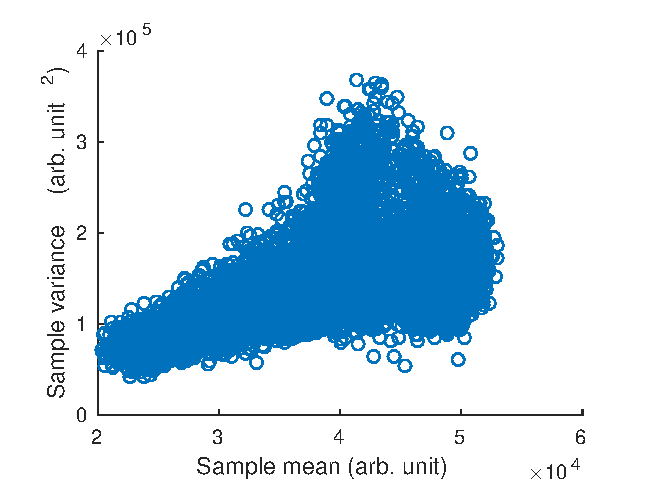
\includegraphics[width=1\textwidth]{figures/meanVar/scatter1.eps}
		\caption{Sample of 7\,968 points}
	\end{subfigure}
	\begin{subfigure}[b]{0.45\textwidth}
		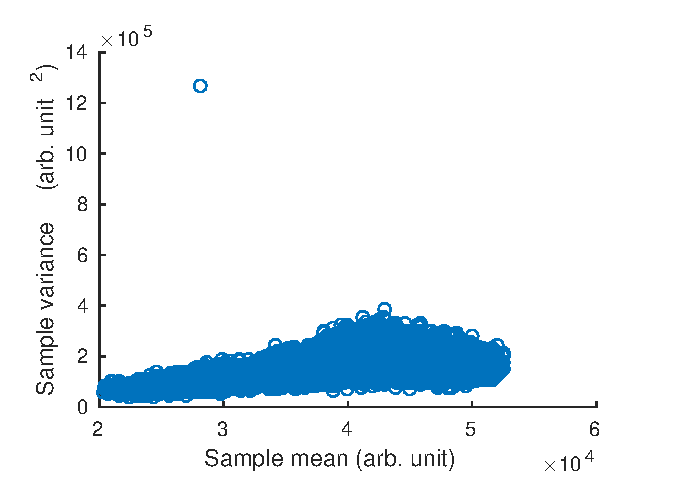
\includegraphics[width=1\textwidth]{figures/meanVar/scatter2.eps}
		\caption{Another sample of 7\,968 points}
	\end{subfigure}
	\caption{Scatter plots of the sample variance-mean pairs of a sample of pixel's grey values.}
	\label{fig:scatterMeanVar}
\end{figure}

\section{Weighted Least Squares}
\subsection{Theory}
The sample variance of the grey values is a random variable, thus itself has uncertainty. Weighted least squares can be used to take into consideration the uncertainty of the sample variance. This can be done by giving low weights to data points with high uncertainty on the grey value variance.

Let $S_i^2$ and $\sigma_i^2$ be the sample variance and true variance, respectively, of the $i$th pixel's grey value for $i=1,2,\dotdotdot,m$ and $m=1\,996^2$. The sample variance has a sampling distribution such that \cite[pp.~195-198]{rice2009mathematical}
\begin{equation}
U_i=\frac{(n-1)S_i^2}{\sigma_i^2}\sim\chi_{n-1}^2
\end{equation}
where $n=100$ is the number of samples used in estimating the variance. The variance is then
\begin{equation*}
2(n-1)=\frac{(n-1)^2}{\sigma_i^4}\variance\left(S_i^2\right)
\end{equation*}
thus
\begin{equation}
\variance\left(S_i^2\right)=\frac{2\sigma_i^4}{n-1} \ .
\end{equation}

A good weight for pixel $i$, $w_i$, would be one which is proportional to the precision, or reciprocal of the variance, of $S_i^2$. $\sigma_i^2$ is generally unknown but can be estimated using $S_i^2$. By doing so, the weights for each grey value was chosen to be
\begin{equation}
w_i \propto \frac{1}{\left(S_i^2\right)^2} \ .
\end{equation}

The weights can be introduced into the least squares problem. Let $Y_1,Y_2,\dotdotdot,Y_m$ and $x_1,x_2,\dotdotdot,x_m$ be the sample variance and mean of the grey values respectively. Let $\vect{x}_1,\vect{x}_2,\dotdotdot,\vect{x}_m$ be the $p$ length feature vectors of the sample mean of the grey values. For example the feature vectors can contain polynomials such that
\begin{equation*}
\vect{x}_i=
\begin{pmatrix}
	1\\x_i\\x_i^2\\\vdots\\x_i^{p-1}
\end{pmatrix} \ .
\end{equation*}
Let $Y_i$ and $x_i$ have a linear relationship such that
\begin{equation}
Y_i = \left(\vect{x}_i\right)\T\vectGreek{\beta} + \epsilon_i
\end{equation}
where $\vectGreek{\beta}$ is a $p$ length parameter vector and $\epsilon_i\sim\normal(0,\sigma_{\epsilon}^2)$ for i.i.d.~$i=1,2,\dotdotdot,m$. The weighted least squares is an optimisation problem where the objective $T$ is minimized by varying $\vectGreek{\beta}$
\begin{equation}
T =
\frac{\sum_{i=1}^mw_i\left(Y_i-\left(\vect{x}_i\right)\T\vectGreek{\beta}\right)^2}
{\sum_{i=1}^mw_i} \ .
\end{equation}
This can be expanded
\begin{equation*}
T =
\frac{\sum_{i=1}^mw_i\left(Y_i-2Y_i\vectGreek{\beta}\T\vect{x}_i+\vectGreek{\beta}\T\vect{x}_i\left(\vect{x}_i\right)\T\vectGreek{\beta}\right)}
{\sum_{i=1}^mw_i} \ .
\end{equation*}
Using the properties of the trace
\begin{equation*}
T =
\frac{\sum_{i=1}^mw_i\left(Y_i-2Y_i\trace\left(\vectGreek{\beta}\T\vect{x}_i\right)+\trace\left(\vectGreek{\beta}\T\vect{x}_i\left(\vect{x}_i\right)\T\vectGreek{\beta}\right)\right)}
{\sum_{i=1}^mw_i}
\end{equation*}
the differential with respect to $\vectGreek{\beta}$, using the results in Appendix \ref{chapter:matrixCalculus}, is
\begin{equation*}
\nabla_{\vectGreek{\beta}}T = \frac{-2\sum_{i=1}^mw_iY_i\vect{x}_i+2\sum_{i=1}^mw_i\vect{x}_i\left(\vect{x}_i\right)\T\vectGreek{\beta}}{\sum_{i=1}^mw_i} \ .
\end{equation*}
Setting the differential to $\vect{0}$, the value of $\vectGreek{\beta}$ which minimises the objective is 
\begin{equation}
\widehat{\vectGreek{\beta}}=\left[\sum_{i=1}^mw_i\vect{x}_i\left(\vect{x}_i\right)\T\right]^{-1}\sum_{i=1}^mw_i\vect{x}_iY_i \ .
\end{equation}

Assuming $Y_1,Y_2,\dotdotdot,Y_m$ are independent and have constant variance $\sigma_\epsilon^2$, the covariance of $\widehat{\vectGreek{\beta}}$ is
\begin{multline}
\cov\left[\widehat{\vectGreek{\beta}}\right]=\matr{\Sigma}_{\widehat{\vectGreek{\beta}}}=
\sigma_\epsilon^2\left[\sum_{i=1}^mw_i\vect{x}_i\left(\vect{x}_i\right)\T\right]^{-1}\left[\sum_{i=1}^mw_i\vect{x}_i\right]
\\
\left[\sum_{i=1}^mw_i\left(\vect{x}_i\right)\T\right]\left[\sum_{i=1}^mw_i\vect{x}_i\left(\vect{x}_i\right)\T\right]^{-1} \ .
\end{multline}
$\sigma_\epsilon^2$ can be estimated using the weighted mean squared error
\begin{equation}
\widehat{\sigma}_\epsilon^2=\frac{\sum_{i=1}^mw_i\left[Y_i-\left(\vect{x}_i\right)\T\widehat{\vectGreek{\beta}}\right]^2}{\sum_{i=1}^mw_i} \ .
\end{equation}

After estimating $\vectGreek{\beta}$ and $\sigma_\epsilon^2$ and given a data point $\vect{x}_{\textup{test}}$, the predicted grey value variance is
\begin{equation}
\widehat{Y}=\left(\vect{x}_{\textup{test}}\right)\T\widehat{\vectGreek{\beta}} + \epsilon_{\textup{test}}
\end{equation}
with expectation
\begin{equation}
\expectation\left[{\widehat{Y}}\right]=\left(\vect{x}_{\textup{test}}\right)\T\widehat{\vectGreek{\beta}}
\end{equation}
and variance
\begin{equation}
\variance\left[\widehat{Y}\right]=\left(\vect{x}_{\textup{test}}\right)\T\matr{\Sigma}_{\widehat{\vectGreek{\beta}}}\vect{x}_{\textup{test}}+\sigma_\epsilon^2
\end{equation}
where $\widehat{\sigma}_\epsilon^2$ can be used in the estimation of $\variance\left(\widehat{Y}\right)$.

\subsection{Methods}
Polynomial features for the sample mean were constructed up to order $k=6$. The weighted linear regression was then fitted. Before fitting the linear regression, the weights were normalized to have a maximum of 1. Furthermore, each feature was normalized to have mean 0 and standard deviation 1. Afterwards, a constant of 1 was appended to each feature vector to model the intercept of the linear regression.

In addition, the BIC was calculated given as
\begin{equation}
\text{BIC} = m\left(\ln2\pi+\ln\widehat{\sigma}_\epsilon^2+1\right)+(k+1)\ln{m}
\end{equation}
for each polynomial order and repeated for 40 different bootstrap samples. A bootstrap sample was obtained by sampling $m$ times without replacement from the original dataset. 

\subsection{Results}
The weighted least squares with polynomial features were fitted successfully as shown in Figure \ref{fig:weightedLS_polynomials}. It appeared successful because the regression goes through the majority of the mean and variance pairs. It was unusual to note that the prediction variance for the 6th order polynomial blew up, further investigation will be needed to explain such behaviour.

The BIC, as shown in Figure \ref{fig:weightedLS_BIC}, favoured high order polynomials. Because the BIC favoured more complicated models, this suggested that fitting polynomial features was not a good model. The BIC aimed to seek more and more polynomials so that the model becomes more similar to the true model. 

\begin{figure}
	\centering
	\begin{subfigure}{0.45\textwidth}
		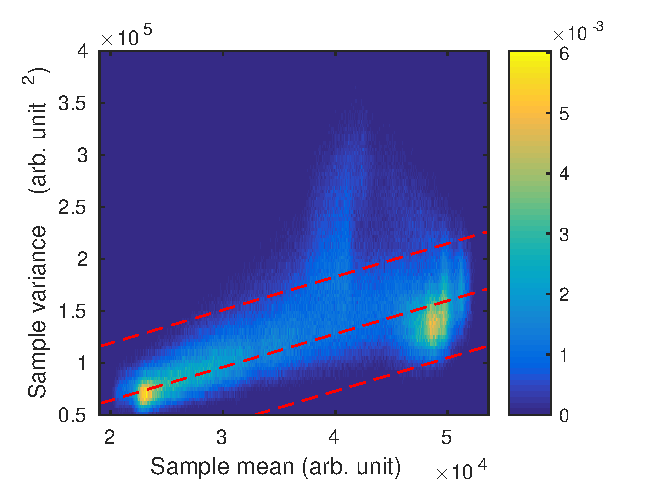
\includegraphics[width=\textwidth]{figures/meanVar/order1.eps}
		\caption{Order 1}
	\end{subfigure}
	\begin{subfigure}{0.45\textwidth}
		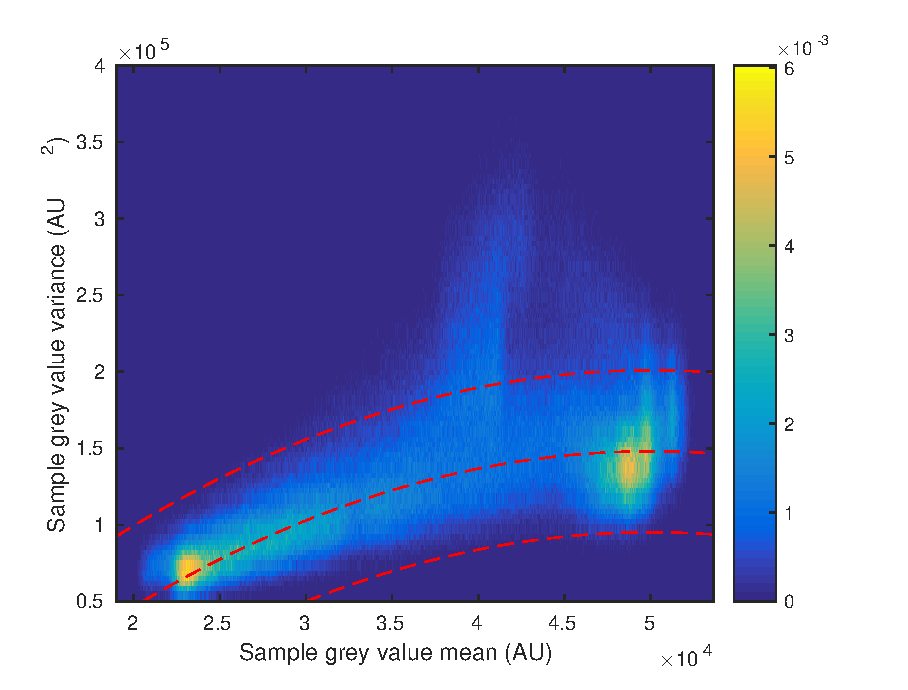
\includegraphics[width=\textwidth]{figures/meanVar/order2.eps}
		\caption{Order 2}
	\end{subfigure}
	\begin{subfigure}{0.45\textwidth}
		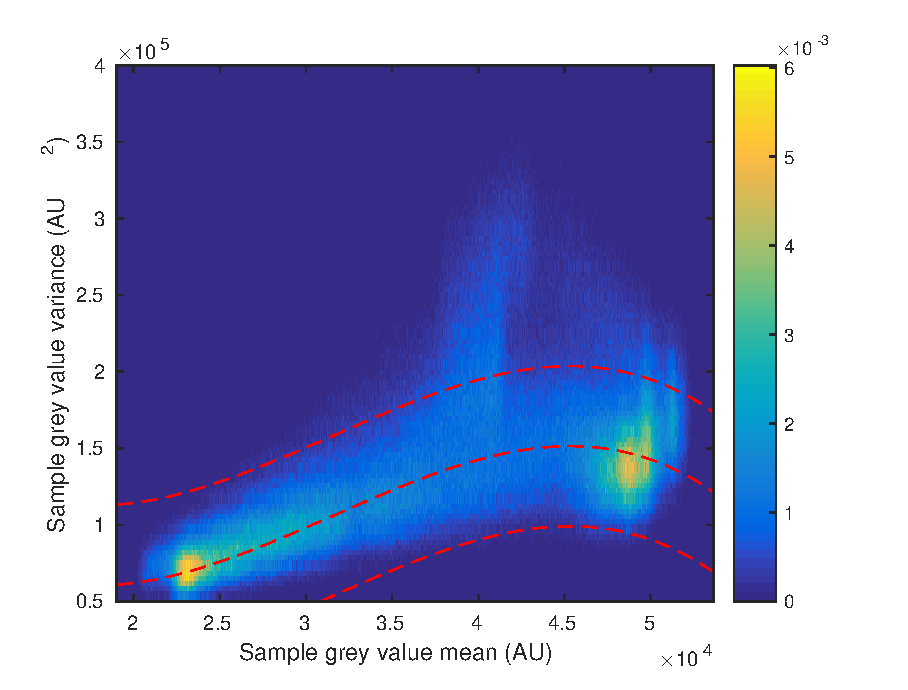
\includegraphics[width=\textwidth]{figures/meanVar/order3.eps}
		\caption{Order 3}
	\end{subfigure}
	\begin{subfigure}{0.45\textwidth}
		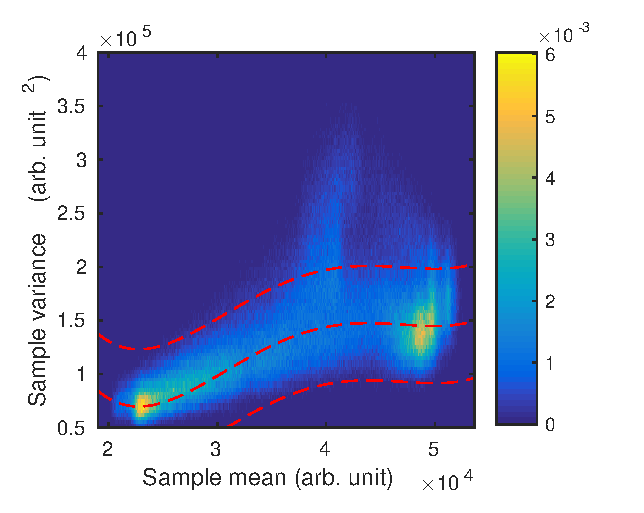
\includegraphics[width=\textwidth]{figures/meanVar/order4.eps}
		\caption{Order 4}
	\end{subfigure}
	\begin{subfigure}{0.45\textwidth}
		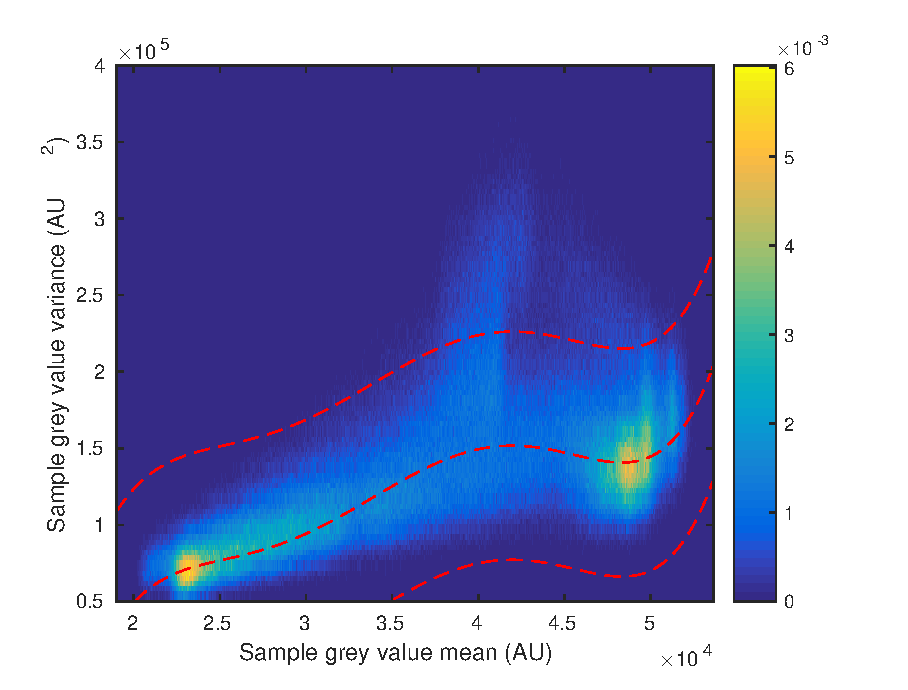
\includegraphics[width=\textwidth]{figures/meanVar/order5.eps}
		\caption{Order 5}
	\end{subfigure}
	\begin{subfigure}{0.45\textwidth}
		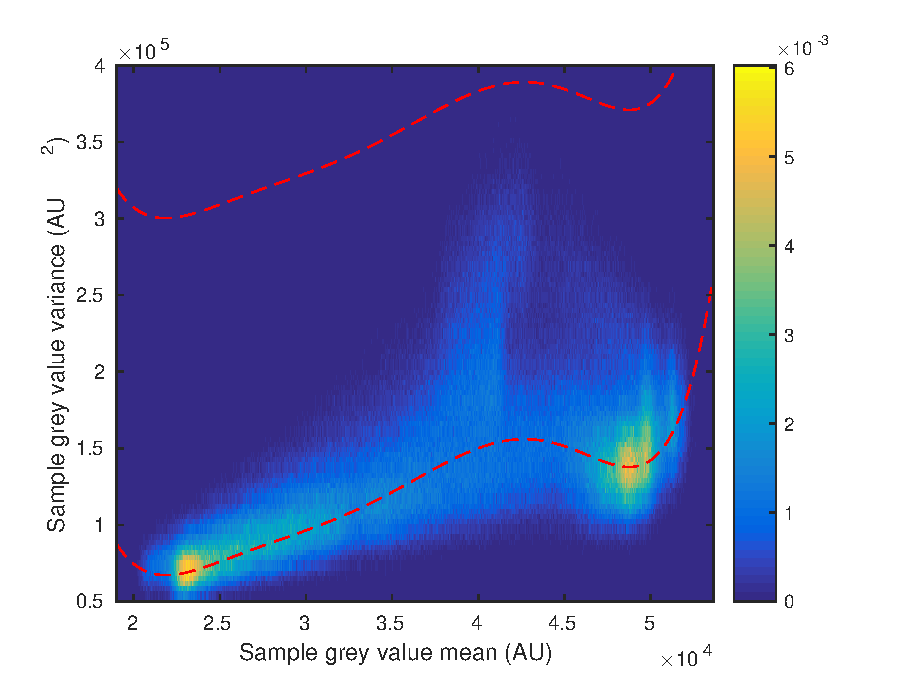
\includegraphics[width=\textwidth]{figures/meanVar/order6.eps}
		\caption{Order 6}
	\end{subfigure}
	\caption{Frequency density of the sample mean and variance of the grey values. Weighted least squares with polynomial features was fitted. The (red) dotted line represent the 95\% prediction interval.}
	\label{fig:weightedLS_polynomials}
\end{figure}

\begin{figure}
	\centering
	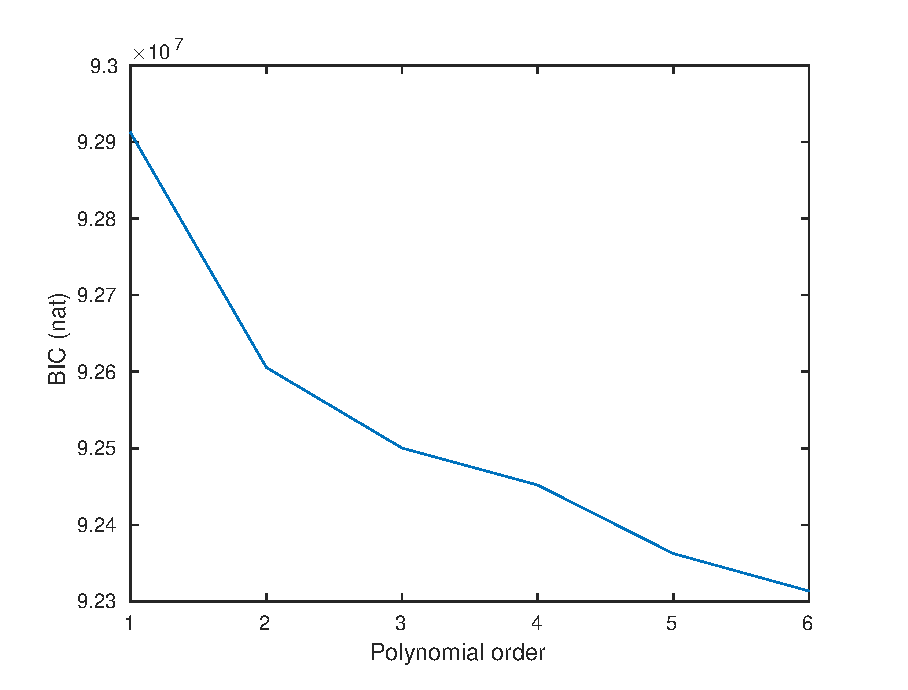
\includegraphics[width=0.75\textwidth]{figures/meanVar/polynomialBIC.eps}
	\caption{BIC, for 40 different bootstrap samples, for fitting weighted least squares with polynomial features on the sample mean sample variance pairs.}
	\label{fig:weightedLS_BIC}
\end{figure}

\section{Subsampling Least Squares}
\subsection{Methods}
From the previous chapter, it was clear there were 3 materials, the 3D printed sample, background and foam, which contributed to the peaks in the histogram of the grey values.

The sample mean sample variance pairs were sub-sampled from each of the 3 materials. A 1st and 2nd order weighted linear regression were fitted for each sub-sample. In addition, the BIC was calculated when fitting such weighted regression on 40 bootstrap samples, for each material.

\subsection{Results}

It was clear the mean-variance relationship is material dependent, this can be seen by the different gradients of the separate regressions in Figure \ref{fig:subsample_meanVar}. The BIC, as shown in Table \ref{table:subsample_BIC}, showed that for the 3D printed sample and foam the BIC favours higher order models. However for the background, when taking into consideration the uncertainty, the BIC can favour the 1st order model.

It was unusual to see the prediction variance to blow for the 2nd order model in the background and foam sub-sample data.

\begin{figure}
	\centering
	\begin{subfigure}{0.45\textwidth}
		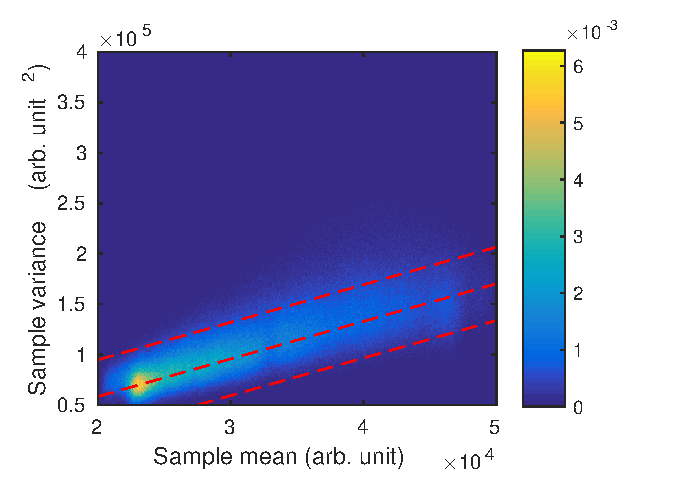
\includegraphics[width=\textwidth]{figures/meanVar/subsample_sample1.eps}
		\caption{Sample- Order 1}
	\end{subfigure}
	\begin{subfigure}{0.45\textwidth}
		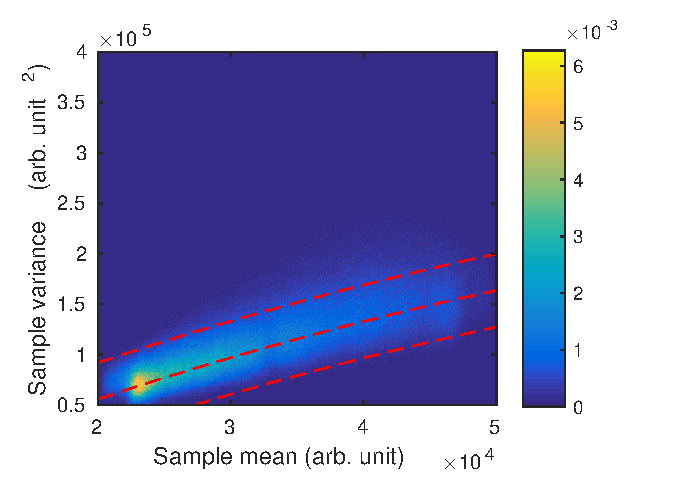
\includegraphics[width=\textwidth]{figures/meanVar/subsample_sample2.eps}
		\caption{Sample - Order 2}
	\end{subfigure}
	\begin{subfigure}{0.45\textwidth}
		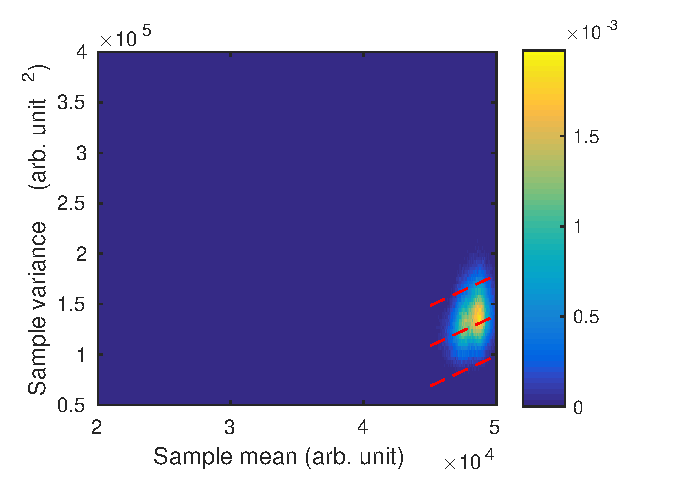
\includegraphics[width=\textwidth]{figures/meanVar/subsample_background1.eps}
		\caption{Background - Order 1}
	\end{subfigure}
	\begin{subfigure}{0.45\textwidth}
		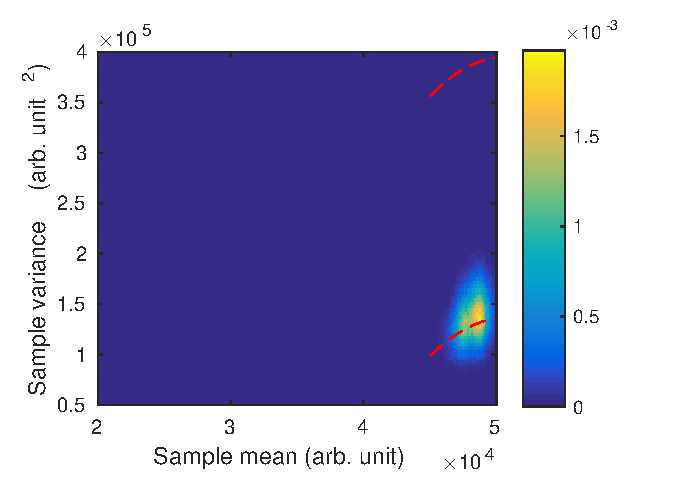
\includegraphics[width=\textwidth]{figures/meanVar/subsample_background2.eps}
		\caption{Background - Order 2}
	\end{subfigure}
	\begin{subfigure}{0.45\textwidth}
		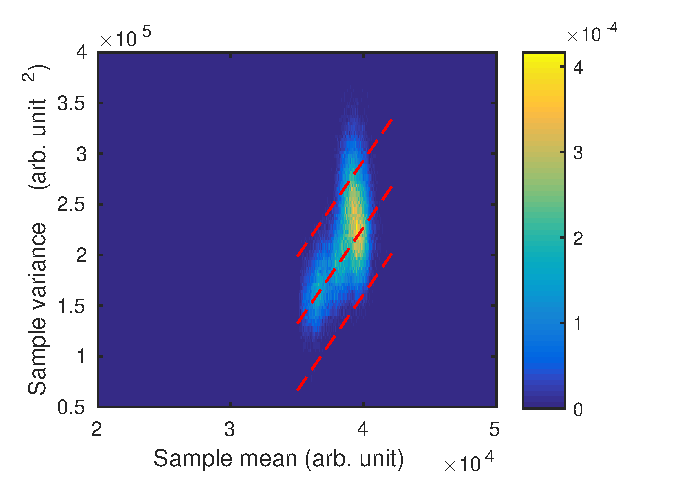
\includegraphics[width=\textwidth]{figures/meanVar/subsample_foam1.eps}
		\caption{Foam - Order 1}
	\end{subfigure}
	\begin{subfigure}{0.45\textwidth}
		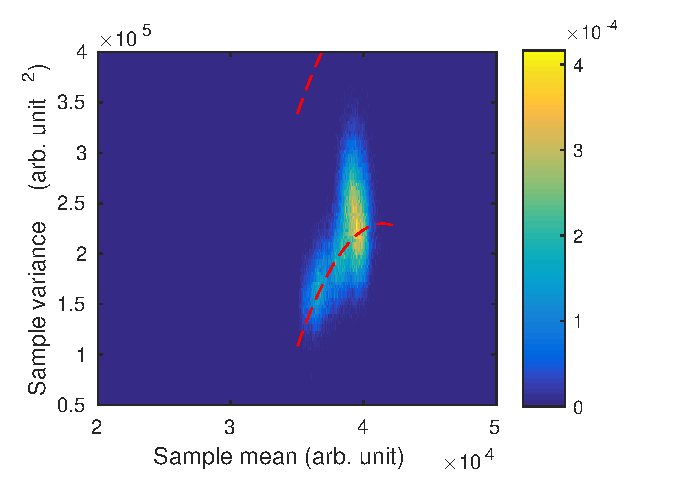
\includegraphics[width=\textwidth]{figures/meanVar/subsample_foam2.eps}
		\caption{Foam - Order 2}
	\end{subfigure}
	\caption{Frequency density of the sample mean and variance of the grey values. Weighted linear regression with polynomial features was fitted on a subsample of sample mean-variance pairs for each material.}
	\label{fig:subsample_meanVar}
\end{figure}

\begin{table}
	\centering
	\begin{tabular}{ c | c c  }
		BIC & Order 1 & Order 2 \\
		\hline
		Sample & $(4.7421\pm0.0003)\times 10^7$ & $(4.7413\pm0.0003)\times 10^7$ \\
		Background & $(4.177\pm0.001)\times 10^6$ & $(4.176\pm0.001)\times 10^6$ \\
		Foam & $(1.5418\pm0.0003)\times 10^6$ & $(1.5403\pm0.0003)\times 10^6$
	\end{tabular}
	\caption{The mean $\pm$ standard deviation of the BIC when fitting weighted least squares with polynomial features on 40 bootstrap samples of the sub-sampled mean-variance pairs for each material.}
	\label{table:subsample_BIC}
\end{table}

\section{Mixture of Linear Regression}

In order to take into consideration the different mean-variance relationship for different materials, a mixture of linear regression was tried to see if it captures the different behaviours.

\subsection{Theory}
A mixture of linear regression was used of the form
\begin{equation}
Y_i\sim
\begin{cases}
\normal\left(\left(\vect{x}_i\right)\T\vectGreek{\beta}_1,\sigma_1^2\right) & \text{if }S_i=1\\ 
\normal\left(\left(\vect{x}_i\right)\T\vectGreek{\beta}_2,\sigma_2^2\right) & \text{if }S_i=2\\
\qquad\qquad\vdots\\
\normal\left(\left(\vect{x}_i\right)\T\vectGreek{\beta}_q,\sigma_q^2\right) & \text{if }S_i=q\\
\end{cases}
\end{equation}
where $S_i$ is a latent variable and $\prob\left(S_i=r\right)=\pi_r$ for $i=1,2,\dotdotdot,m$ and $r=1,2,\dotdotdot,q$.

The likelihood is
\begin{equation*}
L=\prod_{i=1}^m\sum_{j=1}^qp_{Y|S}\left(y_i|S_i=j\right)\pi_j
\end{equation*}
thus the log likelihood is
\begin{equation*}
\ln{L}=\sum_{i=1}^m\ln\left[
\sum_{j=1}^qp_{Y|S}\left(y_i|S_i=j\right)\pi_j
\right]
\end{equation*}
\begin{equation}
\ln{L}=\sum_{i=1}^m\ln\left[
\sum_{j=1}^q \frac{\pi_j}{\sqrt{2\pi}\sigma_j}\exp\left(-\frac{1}{2}\left(\frac{y_i-\left(\vect{x}_i\right)\T\vectGreek{\beta}_j}{\sigma_j}\right)^2\right) 
\right] \ .
\end{equation}
Such a log likelihood can be maximised by using the EM algorithm \cite{dempster1977maximum}, by treating $S_i$ as a random latent variable \cite[pp.~260-261]{barber2012bayesian}.

In the E step, the posterior distribution is used to put a prediction on the latent variables $S_i$ for $i=1,2,\dotdotdot,m$ given estimates of the parameters $\vectGreek{\beta}_j$, $\sigma_j^2$ and $\pi_j$ for $j=1,2,\dotdotdot,q$. The posterior distribution is given as
\begin{equation*}
r_{i,j}=\prob\left(S_i=j|Y_i=y_i\right)=\frac
{p_{Y|S}\left(y_i|S_i=j\right)\pi_j}
{\sum_{j'=1}^qp_{Y|S}\left(y_i|S_i=j'\right)\pi_j}
\end{equation*}
\begin{equation}
r_{i,j}=\prob\left(S_i=j|Y_i=y_i\right)=\dfrac
{\dfrac{\pi_j}{\sqrt{2\pi}\sigma_j}\exp\left[-\frac{1}{2}\left(\dfrac{y_i-\left(\vect{x}_i\right)\T\vectGreek{\beta}_j}{\sigma_j}\right)^2\right] }
{\sum_{j'=1}^q\dfrac{\pi_{j'}}{\sqrt{2\pi}\sigma_{j'}}\exp\left[-\frac{1}{2}\left(\dfrac{y_i-\left(\vect{x}_i\right)\T\vectGreek{\beta}_{j'}}{\sigma_{j'}}\right)^2\right] }
\end{equation}
and such a quantity is called the responsibility of the $i$th data belonging to the $j$th model.

In the M step, the estimations of the  parameters $\vectGreek{\beta}_j$, $\sigma_j^2$ and $\pi_j$ for $j=1,2,\dotdotdot,q$ are updated, using the maximum log likelihood, given the responsibilities $r_{i,j}$ for $i=1,2,\dotdotdot,m$. The regression parameters are updated by
\begin{equation}
\widehat{\vectGreek{\beta}}_j
=
\left[\sum_{i=1}^{m}r_{i,j}
\vect{x}_i\left(\vect{x}_i\right)\T\right]^{-1}
\left[\sum_{i=1}^{m}
r_{i,j}
y_i\vect{x}_i\right]
\end{equation}
and this is weighted least squares where the weights are the responsibilities on model $j$. For the rest of the parameters
\begin{equation}
\widehat{\sigma}_j^2
=
\frac{\sum_{i=1}^{m}
r_{i,j}\left({y_i-\left(\vect{x}_i\right)\T\vectGreek{\beta}_j}\right)^2}
{\sum_{i=1}^{m}r_{i,j}}
\end{equation}
and this is the weighted mean squared error.  Finally
\begin{equation}
\widehat{\pi}_j = \sum_{i=1}^m\frac{r_{i,j}}{m}
\end{equation}
and this is the average responsibility. The proofs for the M step can be found in Appendix \ref{section:Mstep}.

\subsection{Methods}

In this project, only a mixture of 1st order linear regression was considered. The EM algorithm was initialised by assigning random responsibilities for all models and data points in the E step. The number of mixture was set to $q=3$ to see if this model captured the 3 materials. 50 EM steps were used.

To make the EM algorithm run properly without problems, a random sample of 10\,000 sample mean-variance pairs was used in fitting the mixture model.

\subsection{Results}
It was verified that the EM algorithm always increased the log likelihood at every EM step, as can be seen in Figure \ref{fig:mixture_lnL}.

The resulting fit, as shown in Figure \ref{fig:mixture_histogram}, did not capture the 3 different materials. This is because the mixture probabilities, $\pi_1,\pi_2,\pi_3$, do not depend on the sample-mean of the grey values. For example, low grey values are more likely to be from the sample.

\begin{figure}
	\centering	
	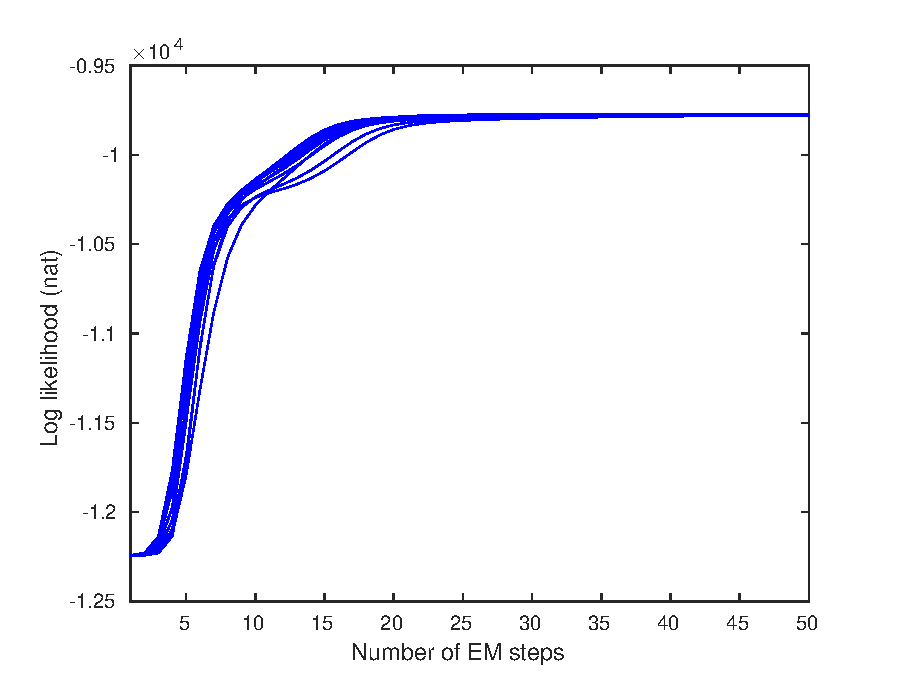
\includegraphics[width=0.75\textwidth]{figures/meanVar/mixture_lnL.eps}
	\caption{The log likelihood of the mixture of linear regressions at every EM step for 10 different initial values.}
	\label{fig:mixture_lnL}
\end{figure}

\begin{figure}
	\centering	
	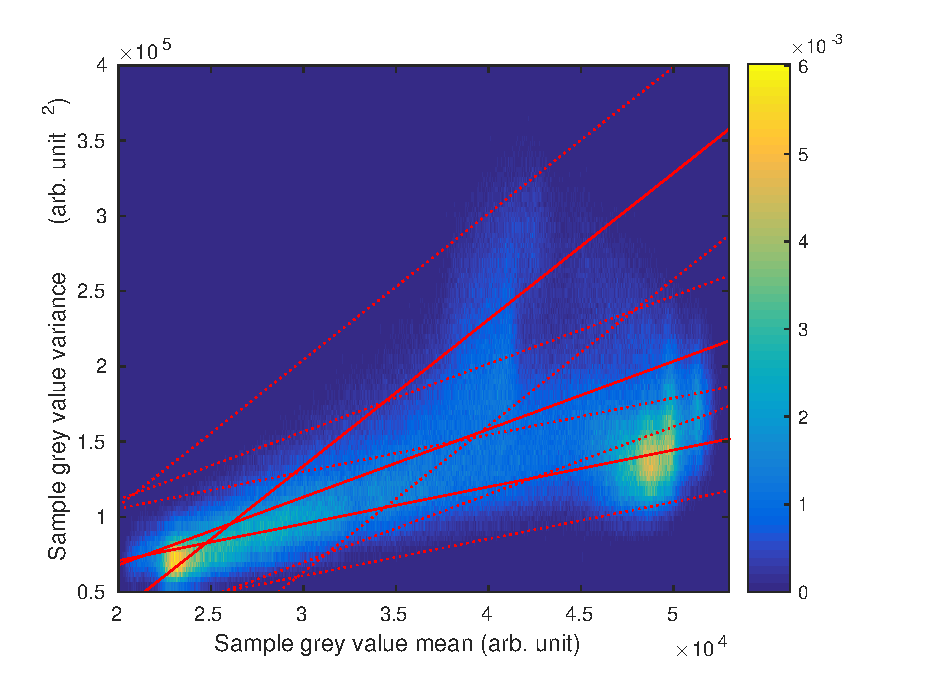
\includegraphics[width=0.75\textwidth]{figures/meanVar/mixture_histogram.eps}
	\caption{Fitting a mixture of 3 linear regressions on the sample mean-variance data.}
	\label{fig:mixture_histogram}
\end{figure}

\section{Distance Weighted Least Squares}
\subsection{Methods}
Weighted least squares was used where the weights depended on some distance from some particular grey value. 3 independent weighted least squares were used where the weights are
\begin{equation}
w_i=\exp\left[-\frac{1}{2}\left(\frac{x_i-\mu_j}{\sigma_j}\right)^2\right] \ ,
\end{equation}
$\mu_j$ was found using $k$-means in the sample-mean grey value space and $\sigma_j$ is a predefined constant, called the Gaussian width.

\subsection{Results}
The model captured the 3D printed sample and foam well because the regression captured the shape of the histogram. However for the background, the regression had a negative gradient as a result of being influenced by lower sample grey values from the foam and 3D printed sample.

For higher Gaussian widths, the regression became an ordinary least squares regression because all the data points have approximately equal weights.

\begin{figure}
	\centering
	\begin{subfigure}{0.45\textwidth}
		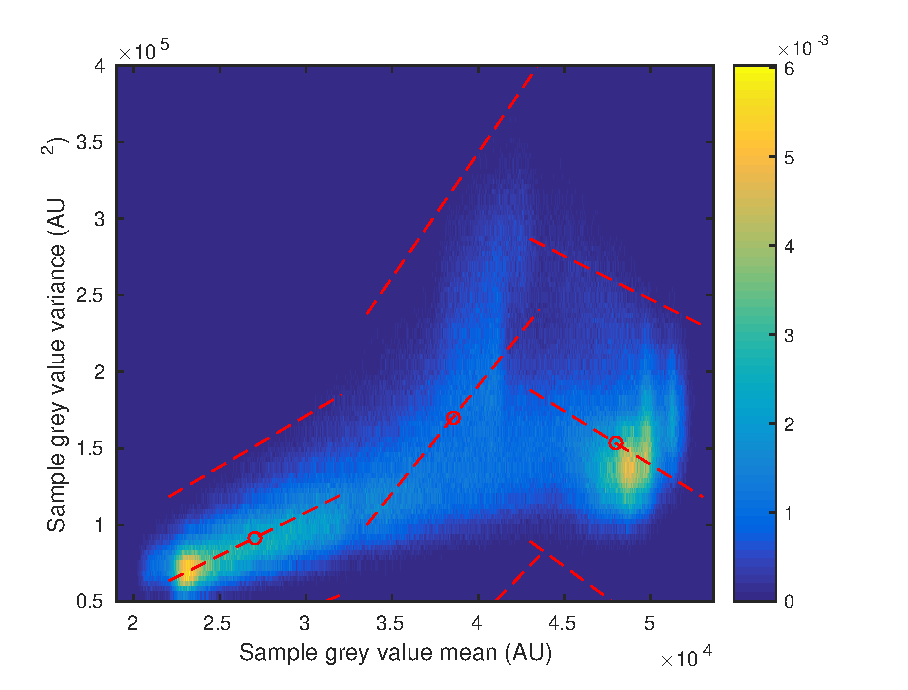
\includegraphics[width=\textwidth]{figures/meanVar/gaussian_1.eps}
		\caption{$\sigma=10^2$}
	\end{subfigure}
	\begin{subfigure}{0.45\textwidth}
		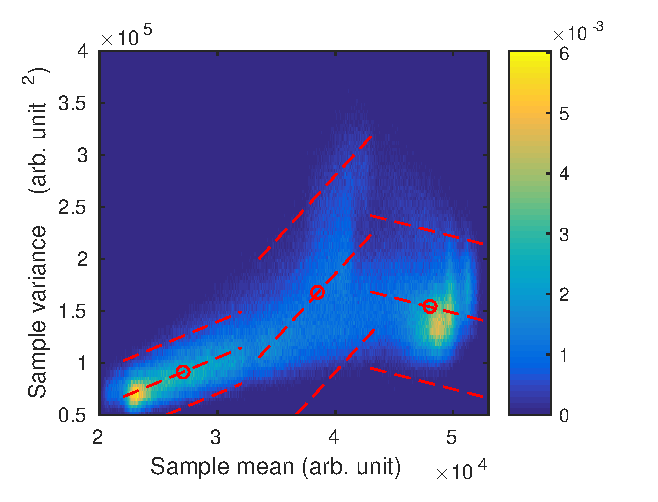
\includegraphics[width=\textwidth]{figures/meanVar/gaussian_2.eps}
		\caption{$\sigma=10^3$}
	\end{subfigure}
	\begin{subfigure}{0.45\textwidth}
		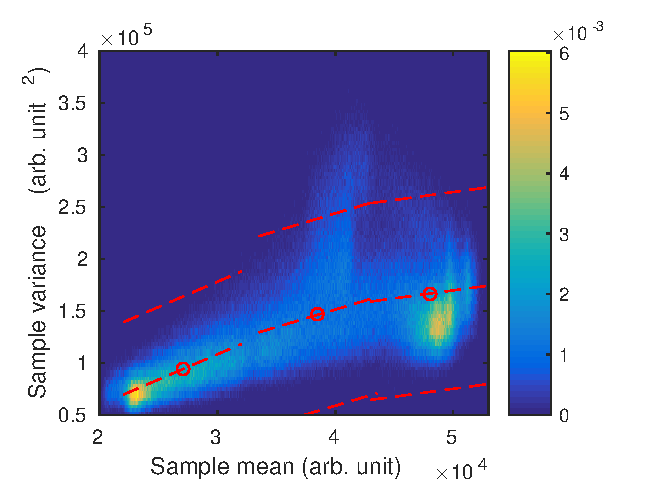
\includegraphics[width=\textwidth]{figures/meanVar/gaussian_3.eps}
		\caption{$\sigma=10^4$}
	\end{subfigure}
	\begin{subfigure}{0.45\textwidth}
		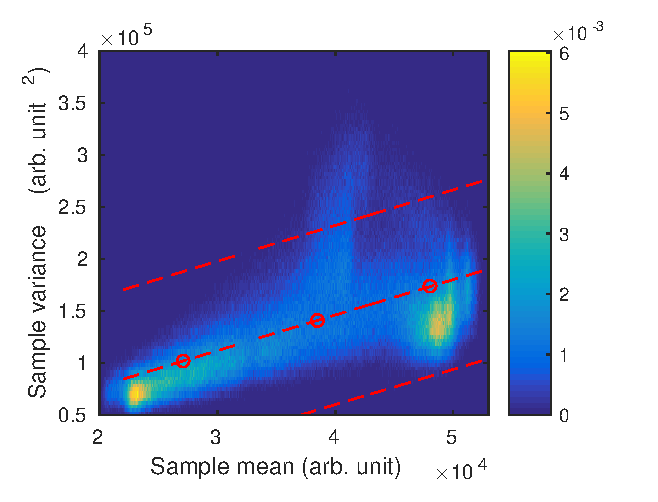
\includegraphics[width=\textwidth]{figures/meanVar/gaussian_4.eps}
		\caption{$\sigma=10^5$}
	\end{subfigure}
	\caption{3 independent Gaussian weighted least squares regressions. The weights depended on the distance from the $k$-means sample mean grey values and some width $\sigma$.}
\end{figure}

\chapter{Latent Variable Model}

\section{Principal Component Analysis}
By estimating the covariance matrix of the individual pixel's grey values, sources of (orthgonal) variance can be estimated. This can be done investigating eigendecomposition representation of the sample covariance matrix. A lot of the linear algebra can be reviewed in undergraudate maths text book such as \cite{riley2006mathematical}.

\subsection{Theory}
Suppose the $p\times p$ covariance matrix $\matr{\Sigma}$ has eigenvalues $\lambda_i$ and eigenvector $\vectGreek{\phi}_i$ for $i=1,2,\dotdotdot,p$. Then the eigenvectors and eigenvalues are related by
\begin{equation}
\matr{\Sigma}\vectGreek{\phi}_i = \lambda_i\vectGreek{\phi}_i \ .
\label{eq:eigenvector_eigenvalue_forCovariance}
\end{equation}
A closure can be form by pre-multiplying both sides by $\vectGreek{\phi}_j\T$ so that
\begin{align*}
\vectGreek{\phi}_j\T \matr{\Sigma}\vectGreek{\phi}_i &= \lambda_i\vectGreek{\phi}_j\T\vectGreek{\phi}_i \\
\left(\matr{\Sigma}\T \vectGreek{\phi}_j \right)\T\vectGreek{\phi}_i &= \lambda_i\vectGreek{\phi}_j\T\vectGreek{\phi}_i \ .
\end{align*}
But given the covariance matrix is symmetric, $\matr{\Sigma}=\matr{\Sigma}\T$, and $\lambda_j$ is the corresponding eigenvalue of the eigenvector $\vectGreek{\phi}_j$, then
\begin{align*}
\left(\lambda_j\vectGreek{\phi}_j \right)\T\vectGreek{\phi}_i &= \lambda_i\vectGreek{\phi}_j\T\vectGreek{\phi}_i \\
\lambda_j\vectGreek{\phi}_j\T\vectGreek{\phi}_i &= \lambda_i\vectGreek{\phi}_j\T\vectGreek{\phi}_i \ .
\end{align*}
As long as $\lambda_i\neq\lambda_j$ for $i\neq j$, then $\vectGreek{\phi}_j\T\vectGreek{\phi}_i=0$. Therefore all eigenvalues in the covariance matrix are orthogonal to each other.

Equation \eqref{eq:eigenvector_eigenvalue_forCovariance} can be extended to include all eigenvectors and eigenvalues such that
\begin{equation}
\matr{\Sigma}
	\begin{pmatrix}
		\uparrow & \uparrow & & \uparrow \\
		\vectGreek{\phi}_1 & \vectGreek{\phi}_2 &\cdots& \vectGreek{\phi}_p \\
		\downarrow & \downarrow & & \downarrow \\
	\end{pmatrix}
=
	\begin{pmatrix}
		\uparrow & \uparrow & & \uparrow \\
		\lambda_1\vectGreek{\phi}_1 & \lambda_2\vectGreek{\phi}_2 &\cdots& \lambda_p\vectGreek{\phi}_p \\
		\downarrow & \downarrow & & \downarrow \\
	\end{pmatrix} \ .
\end{equation}
Transposing both sides
\begin{equation*}
\begin{pmatrix}
	\leftarrow\vectGreek{\phi}_1\rightarrow \\
	\leftarrow\vectGreek{\phi}_2\rightarrow \\
	\vdots \\
	\leftarrow\vectGreek{\phi}_p\rightarrow
\end{pmatrix}
\matr{\Sigma}
=
\begin{pmatrix}
	\lambda_1 & 0 & \cdots 0 \\
	0 & \lambda_2 & \cdots 0 \\
	\vdots & \vdots & \ddots \\
	0 & 0 & \cdots \lambda_p \\
\end{pmatrix}
\begin{pmatrix}
	\leftarrow\vectGreek{\phi}_1\rightarrow \\
	\leftarrow\vectGreek{\phi}_2\rightarrow \\
	\vdots \\
	\leftarrow\vectGreek{\phi}_p\rightarrow
\end{pmatrix}
\end{equation*}
but because all eigenvectors are orthogonal
\begin{equation*}
\matr{\Sigma}
=
\begin{pmatrix}
		\uparrow & \uparrow & & \uparrow \\
		\vectGreek{\phi}_1 & \vectGreek{\phi}_2 &\cdots& \vectGreek{\phi}_p \\
		\downarrow & \downarrow & & \downarrow \\
\end{pmatrix}
\begin{pmatrix}
	\lambda_1 & 0 & \cdots 0 \\
	0 & \lambda_2 & \cdots 0 \\
	\vdots & \vdots & \ddots \\
	0 & 0 & \cdots \lambda_p \\
\end{pmatrix}
\begin{pmatrix}
	\leftarrow\vectGreek{\phi}_1\rightarrow \\
	\leftarrow\vectGreek{\phi}_2\rightarrow \\
	\vdots \\
	\leftarrow\vectGreek{\phi}_p\rightarrow
\end{pmatrix} \ .
\end{equation*}
This is just a weighted sum of the outer products of the eigenvectors, therefore the eigendecomposition is
\begin{equation}
\matr{\Sigma} = \sum_{i=1}^{p} \lambda_i \vectGreek{\phi}_i \vectGreek{\phi}_i\T \ .
\end{equation}
Because this is a weighted sum, the eigenvectors with the biggest eigenvalue will be most responsible for the covariance matrix. $\vectGreek{\phi}_i$ are called the principle components.

\subsection{Methods}
The 100 images were shrunk with averaging to a size of $100\times100$ pixels using ImageJ \cite{schindelin2012fiji}. The sample covariance matrix, of the pixel's grey values, was calculated using the maximum likelihood estimator so that the 6 eigenvectors with the biggest eigenvalues can be obtained. Using 1\,600 bootstrap samples, the sampling distribution of the 6 eigenvalues were sampled.

\subsection{Results}
Figure \ref{fig:initial_PC_eigenvalues} shows the first 6 of the diagonal of the outer product of the individual principle components, they represent the normalised main sources of variance. It was observed that on the first and second principle components, there are sources of variance in the bottom right and top right of the image. This could imply that the sources of variance are not uniformly distributed in the background.

The sampling distribution of the eigenvalues are shown in Figure \ref{fig:initial_PC_eigenvalues}. Quite clearly there were 2 significant sources of variance because the eigenvalues of the first 2 principle components were much larger than zero when comparing it with its interquartile range.

\begin{figure}
	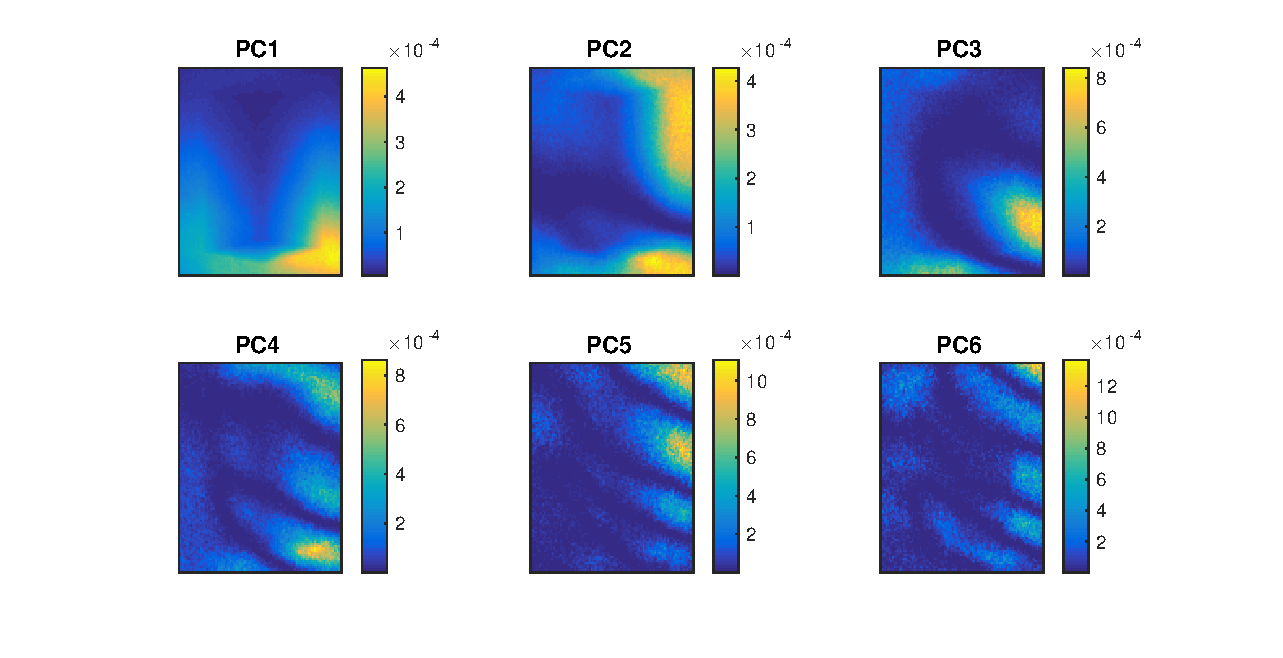
\includegraphics[width=\textwidth]{figures/initial_PCvariance.eps}
	\caption{Normalised variance due to the principle components (1 to 6). The sum of all the values in each figures equal to 1.}
	\label{fig:initial_PCvariance}
\end{figure}

\begin{figure}
	\centering
	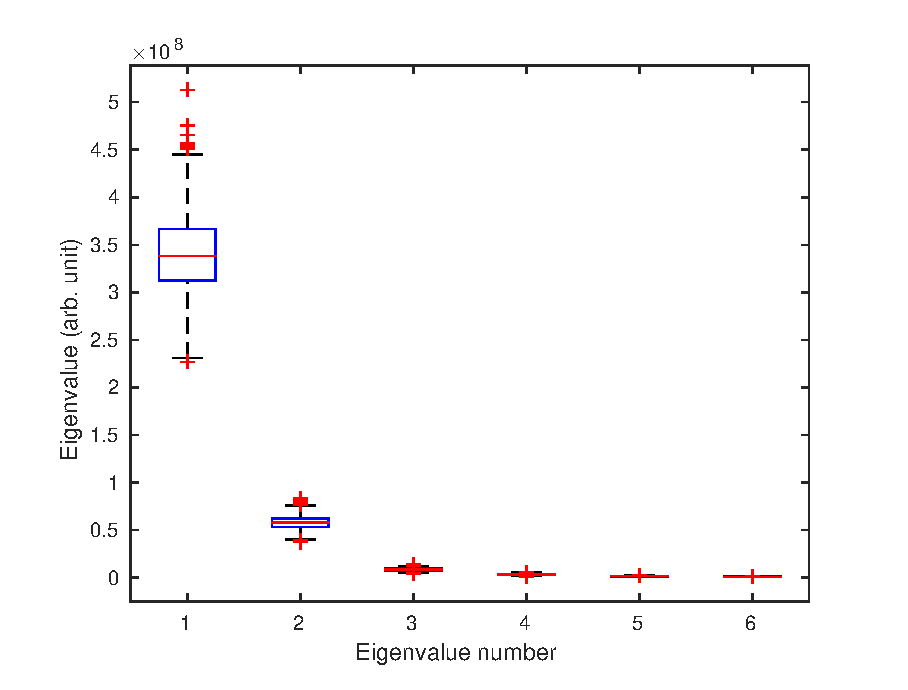
\includegraphics[width=0.75\textwidth]{figures/initial_PC_eigenvalues.eps}
	\caption{Eigenvalues of the sample covariance matrix. 1\,600 bootstrap samples were used.}
	\label{fig:initial_PC_eigenvalues}
\end{figure}

\section{Factor Analysis}
A probabilistic latent model can be used to model the pixel's grey values. These latent variables then can be used to describe the underlining structure, and perhaps sources of variance.

\subsection{Theory}
Let $\vect{Y}$ be a random vector containing $k$ latent variables, called factors, and
\begin{equation}
\vect{Y}\sim\normal\left(\vect{0},\matr{1}\right) \ .
\end{equation}
Let $\vect{e}$ be a random $p$ vector modelling the uncorrelated intrinsic noise such that
\begin{equation}
\vect{e}\sim\normal\left(\vect{0},\matr{\Psi}\right)
\end{equation}
where $\matr{\Psi}$ is a diagonal matrix.

Given a $p\times k$ loading matrix $\matr{\Lambda}$, the observable data $\vect{X}$ can be modelled through
\begin{equation}
\vect{X}=\matr{\Lambda}\vect{Y}+\vect{e}
\end{equation}
thus
\begin{equation}
\vect{X}\sim\normal\left(\vect{0},\matr{\Lambda}\matr{\Lambda}\T+\matr{\Psi}\right) \ .
\end{equation}
As a result there are two sources of variance, factor noise from the $\matr{\Lambda}\matr{\Lambda}\T$ component and the instrinic noise $\matr{\Psi}$. The model can be extended for non-zero mean easily by adding an arbitrary constant.

The conditional distribution of $\vect{X}$ given $\vect{Y}$ can be calculated to be
\begin{equation}
\vect{X}|\vect{Y}\sim\normal\left(\matr{\Lambda}\vect{Y},\matr{\Psi}\right) \ .
\label{eq:factor_analysis_x_given_y_dist}
\end{equation}
Using Bayes' theorem, the conditional distribution of $\vect{Y}$ given $\vect{X}$ can be calculated
\begin{align*}
p_{\vect{Y}|\vect{X}}(\vect{y}|\vect{x}) &\propto p_{\vect{X}|\vect{Y}}(\vect{x}|\vect{y}) p_{\vect{Y}}(\vect{y})
\\
p_{\vect{Y}|\vect{X}}(\vect{y}|\vect{x}) &\propto \exp\left[-\frac{1}{2}\left(\vect{x}-\matr{\Lambda}\vect{y}\right)\T\matr{\Psi}^{-1}\left(\vect{x}-\matr{\Lambda}\vect{y}\right)\right]
\exp\left[-\frac{1}{2}\vect{y}\T\vect{y}\right]
\\
p_{\vect{Y}|\vect{X}}(\vect{y}|\vect{x}) &\propto \exp \left[-\frac{1}{2}\left(-\vect{x}\T\matr{\Psi}^{-1}\matr{\Lambda}\vect{y}-\vect{y}\T\matr{\Lambda}\T\matr{\Psi}^{-1}\vect{x}+\vect{y}\T\matr{\Lambda}\T\matr{\Psi}^{-1}\matr{\Lambda}\vect{y}+\vect{y}\T\vect{y}\right)\right]
\\
p_{\vect{Y}|\vect{X}}(\vect{y}|\vect{x}) &\propto \exp \left[-\frac{1}{2}\left(\vect{y}\T\left(\matr{\Lambda}\T\matr{\Psi}^{-1}\matr{\Lambda}+\matr{1}\right)\vect{y}-2\vect{y}\T\matr{\Lambda}\T\matr{\Psi}^{-1}\vect{x}\right)\right]
\end{align*}
and comparing it with the density function of a general multivariate Normal distribution
\begin{equation}
\vect{Y}|\vect{X}\sim\normal\left(\left(\matr{\Lambda}\T\matr{\Psi}^{-1}\matr{\Lambda}+\matr{1}\right)^{-1}\matr{\Lambda}\T\matr{\Psi}^{-1}\vect{X},\left(\matr{\Lambda}\T\matr{\Psi}^{-1}\matr{\Lambda}+\matr{1}\right)^{-1}\right) \ .
\label{eq:factor_analysis_y_given_x_dist}
\end{equation}

Suppose $\vect{X}=\vect{x}^{(i)}$ was observed for $i=1,2,\dotdotdot,n$, then the likelihood is
\begin{equation}
L=\prod_{i=1}^n\frac{1}{{\|2\pi\left(\matr{\Lambda}\matr{\Lambda}\T+\matr{\Psi}\right)\|}^{1/2}}
\exp\left[-\frac{1}{2}\left(\vect{x}^{(i)}\right)\T\left(\matr{\Lambda}\matr{\Lambda}\T+\matr{\Psi}\right)^{-1}\vect{x}^{(i)}\right] \ .
\end{equation}
The log likelihood is then
\begin{equation*}
\ln{L}=-\frac{n}{2}\ln{\|2\pi\left(\matr{\Lambda}\matr{\Lambda}\T+\matr{\Psi}\right)\|}-\frac{1}{2}\sum_{i=1}^{n}\left(\vect{x}^{(i)}\right)\T\left(\matr{\Lambda}\matr{\Lambda}\T+\matr{\Psi}\right)^{-1}\vect{x}^{(i)}
\end{equation*}
and by using the trace and its properties
\begin{align}
\ln{L}&=-\frac{n}{2}\ln{\|2\pi\left(\matr{\Lambda}\matr{\Lambda}\T+\matr{\Psi}\right)\|}-\frac{1}{2}\sum_{i=1}^{n}\trace\left[\left(\vect{x}^{(i)}\right)\T\left(\matr{\Lambda}\matr{\Lambda}\T+\matr{\Psi}\right)^{-1}\vect{x}^{(i)}\right]
\nonumber \\
\ln{L}&=-\frac{n}{2}\ln{\|2\pi\left(\matr{\Lambda}\matr{\Lambda}\T+\matr{\Psi}\right)\|}-\frac{1}{2}\sum_{i=1}^{n}\trace\left[\left(\matr{\Lambda}\matr{\Lambda}\T+\matr{\Psi}\right)^{-1}\vect{x}^{(i)}\left(\vect{x}^{(i)}\right)\T\right]
\nonumber \\
\ln{L}&=-\frac{n}{2}\ln{\|2\pi\left(\matr{\Lambda}\matr{\Lambda}\T+\matr{\Psi}\right)\|}-\frac{1}{2}\trace\left[\left(\matr{\Lambda}\matr{\Lambda}\T+\matr{\Psi}\right)^{-1}\sum_{i=1}^{n}\vect{x}^{(i)}\left(\vect{x}^{(i)}\right)\T\right] \ .
\end{align}
The loading matrix $\matr{\Lambda}$ and intrinsic noise $\matr{\Psi}$ can be estimated by maximising the log likelihood. This is best done using the expectation maximisation (EM) algorithm. The EM algorithm is an iterative procedure conducting an E step followed by a M step many times till some convergence conditions are met.

The E step estimates the values of the latent variables, $\vect{Y}^{(1)},\vect{Y}^{(2)},\dotdotdot,\vect{Y}^{(n)}$, using the expectation of the conditional distribution of the latent variables given the observed data $\vect{x}^{(1)},\vect{x}^{(2)},\dotdotdot,\vect{x}^{(n)}$. The parameters $\matr{\Lambda}$ and $\matr{\Psi}$ are assumed to be know in this step and are fixed. By using Equation \eqref{eq:factor_analysis_y_given_x_dist}, each latent variable are predicted by the conditional expectation
\begin{equation}
\expectation\left[\vect{Y}^{(i)}|\vect{X}^{(i)}=\vect{x}^{(i)}\right]=\vect{y}^{(i)} = \left(\matr{\Lambda}\T\matr{\Psi}^{-1}\matr{\Lambda}+\matr{1}\right)^{-1}\matr{\Lambda}\T\matr{\Psi}^{-1}\vect{x}^{(i)}
\end{equation}
for $i=1,2,\dotdotdot,n$. The covariance of the latent variables are estimated by
\begin{equation}
\cov\left[\vect{Y}^{(i)}|\vect{X}^{(i)}=\vect{x}^{(i)}\right]=\matr{\Sigma}_{\vect{Y}} = \left(\matr{\Lambda}\T\matr{\Psi}^{-1}\matr{\Lambda}+\matr{1}\right)^{-1}
\end{equation}

In the E step, the parameters $\matr{\Lambda}$ and $\matr{\Psi}$ are varied to maximise the log likelihood, assuming the latent variables are known and fixed. The objective is to maximise is the condition expectation of the log joint likelihood, that is
\begin{equation}
H = \expectation_{\vect{Y}|\vect{X}}\left[\sum_{i=1}^{n}\ln p_{\vect{X},\vect{Y}}\left(\vect{x}^{(i)},\vect{Y}^{(i)}\right)\right] \ .
\end{equation}
It is given the $\matr{\Lambda}$ and $\matr{\Psi}$ which maximises $H$ is
\begin{equation}
\widehat{\matr{\Lambda}}
=
\left(\sum_{i=1}^n\vect{x}^{(i)}\left(\vect{y}^{(i)}\right)\T\right)\left(n\matr{\Sigma}_{\vect{Y}}+\sum_{i=1}^{n}\vect{y}^{(i)}\left(\vect{y}^{(i)}\right)\T\right)^{-1}
\end{equation}
and
\begin{equation}
\widehat{\matr{\Psi}} =\text{diag}\left[
\frac{1}{n}\sum_{i=1}^{n}\left(
\left(\vect{x}^{(i)}-\matr{\Lambda}\vect{y}^{(i)}\right)
\left(\vect{x}^{(i)}-\matr{\Lambda}\vect{y}^{(i)}\right)\T
\right)
+\matr{\Lambda}\matr{\Sigma}_{\vect{Y}}\matr{\Lambda}\right]\ .
\end{equation}
The proofs for the M step can be found in Appendix \ref{chapter:mStep_factorAnalysis}.

\subsection{Methods}
The data was centred so that the mean of each pixel's gray value was zero. By doing this, factor analysis focuses on modelling the variance of the pixel's gray values.

For a given $k$ number of factors, the EM algorithm was initialized by randomly assigning each element of $\matr{\Lambda}$ to have distribution $\normal(0,(10^3)^2)$. In addition, each diagonal entry of $\matr{\Psi}$ was initialized by sampling from the $\gammaDist(1,10^{-3})$ distribution. This was chosen to have arbitrary large variance so that it covers as much of the parameter space as possible.

The EM algorithm was run many times with different initial values. Because evaluating the log likelihood was expensive, the stopping condition is met when a certain amount of E and M steps were taken. The parameters with the lowest log likelihood was recorded.

The Bayesian information criterion (BIC) was used to select the best $k$ to use. The BIC is given as
\begin{equation}
\BIC=-2\ln L + p(k+1)\ln n \ .
\end{equation}
The data was bootstrapped to assess the uncertainty in the model selection.

\subsection{Results}
$k=1,2,\dotdotdot,15$ were investigated. The EM algorithm was repeated 81 times for each $k$ with a stopping condition of 100 EM steps. The BIC for each $k$ is as shown in Figure \ref{fig:initial_factor_BIC}. The number of factors with the lowest BIC was found to be 8.

The 8 factor variances were isolated and as shown in Figure \ref{fig:initial_factor_factorNoise}, together with the intrinsic variance as shown in Figure \ref{fig:initial_factor_instrinicNoise}. It was interesting to note that in Figure \ref{fig:initial_factor_factorNoise}, there are clusters of high variance in most of the factors. This suggest clusters of high variance can appear in the data randomly, thus the variance of each of the pixel's gray values can depend on each other spatially. In Figure \ref{fig:initial_factor_instrinicNoise}, the shape of the sample can be seen represented by the low intrinsic variance. This was evidence that they may well be a mean and variance relationship.

\begin{figure}
	\centering
	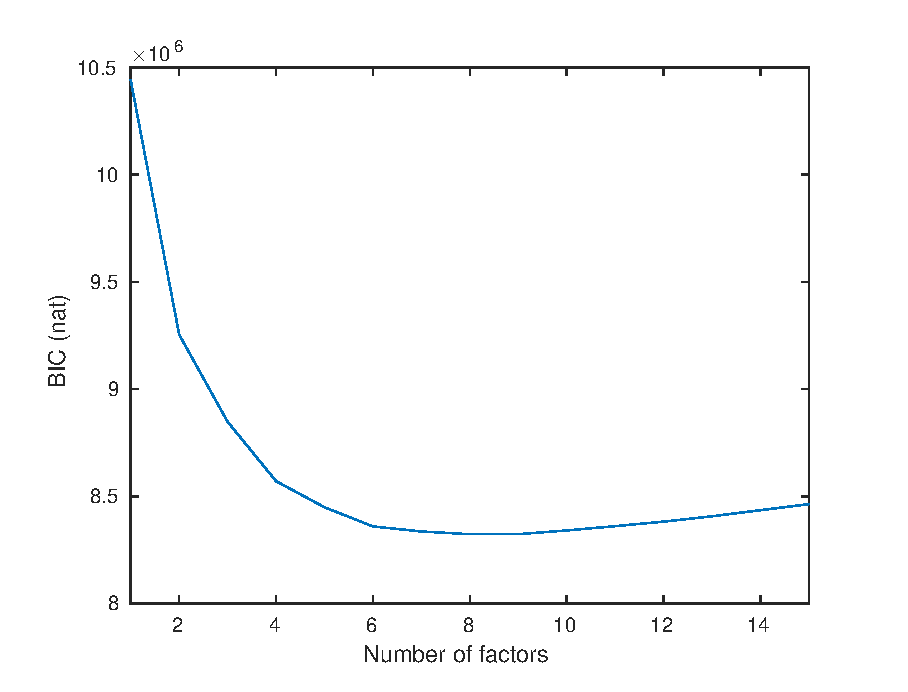
\includegraphics[width=0.75\textwidth]{figures/initial_factor_BIC.eps}
	\caption{BIC for fitting different number of factors onto the data. 81 different initials were used for each $k$ with a stopping condition of 100 EM steps.}
	\label{fig:initial_factor_BIC}
\end{figure}

\begin{figure}
	\centering
	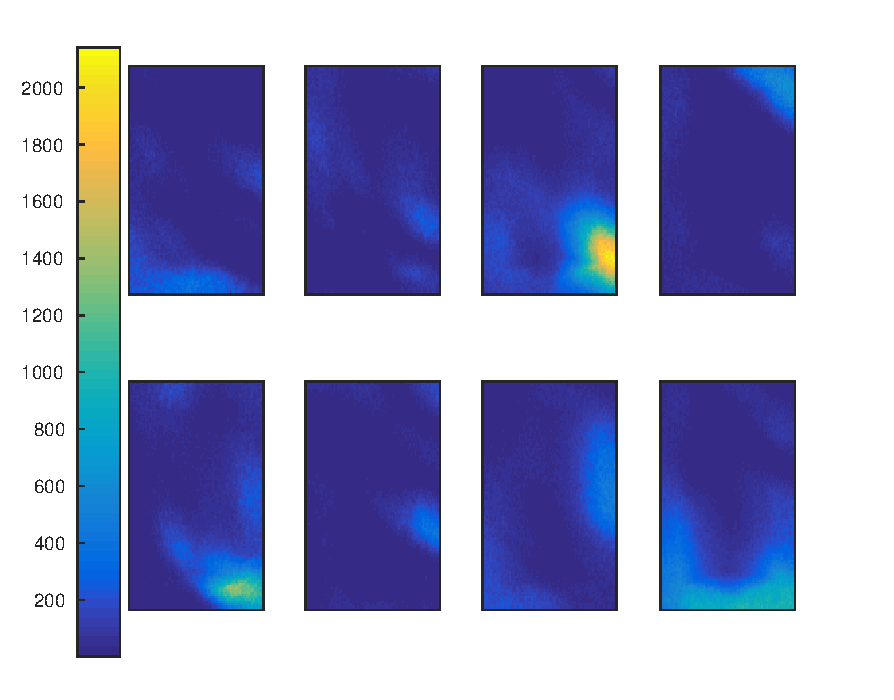
\includegraphics[width=0.75\textwidth]{figures/initial_factor_factorNoise.eps}
	\caption{The 8 individual factor variances with the lowest log likelihood found.}
	\label{fig:initial_factor_factorNoise}
\end{figure}

\begin{figure}
	\centering
	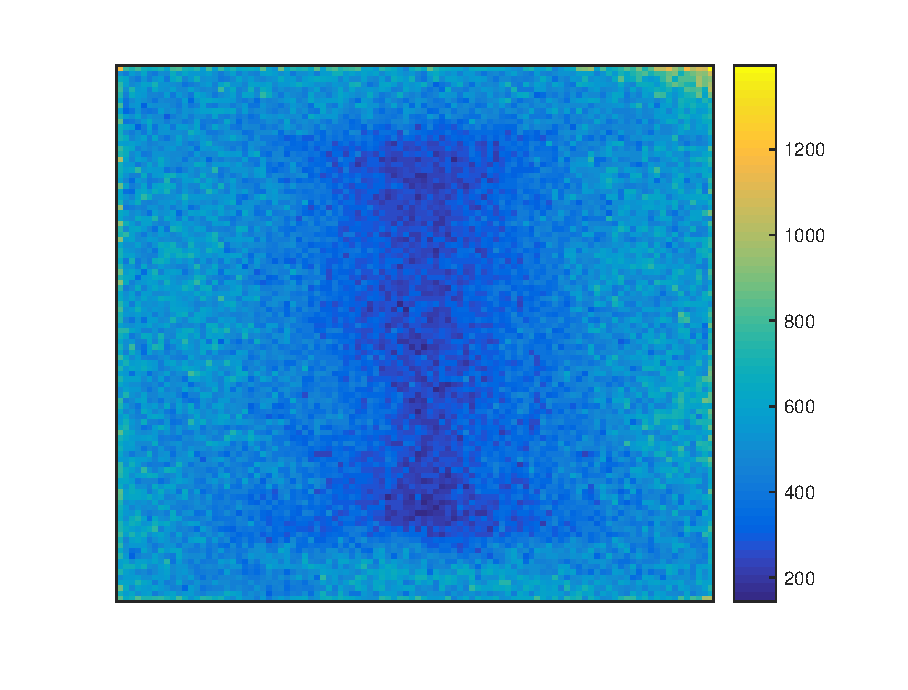
\includegraphics[width=0.75\textwidth]{figures/initial_factor_instrinicNoise.eps}
	\caption{The intrinsic variances with the lowest log likelihood found.}
	\label{fig:initial_factor_instrinicNoise}
\end{figure}

The uncertainty of model selection was assessed by investigating how the BIC and optimal $k$ varied for different bootstrap samples. The BIC for the 99 bootstrap samples is shown in Figure \ref{fig:initial_factor_BIC_bootstrap}. Only one initial value was used for each $k$ to capture the uncertainty if the EM algorithm converges to a global maxima or not. From the figure, quite clearly there was a lot of variability in the BIC and can cause imprecise decisions on model selection. Over all 99 bootstrap samples, the mean and standard deviation optimal $k$ was found to be $10\pm2$ factors.

The main source of error was down to the small sample size. The experiments can be improved if the analysis was done on the full size image rather than downsizing it. When downsizing, there is a risk of tampering the variance of the pixel's grey values.

\begin{figure}
	\centering
	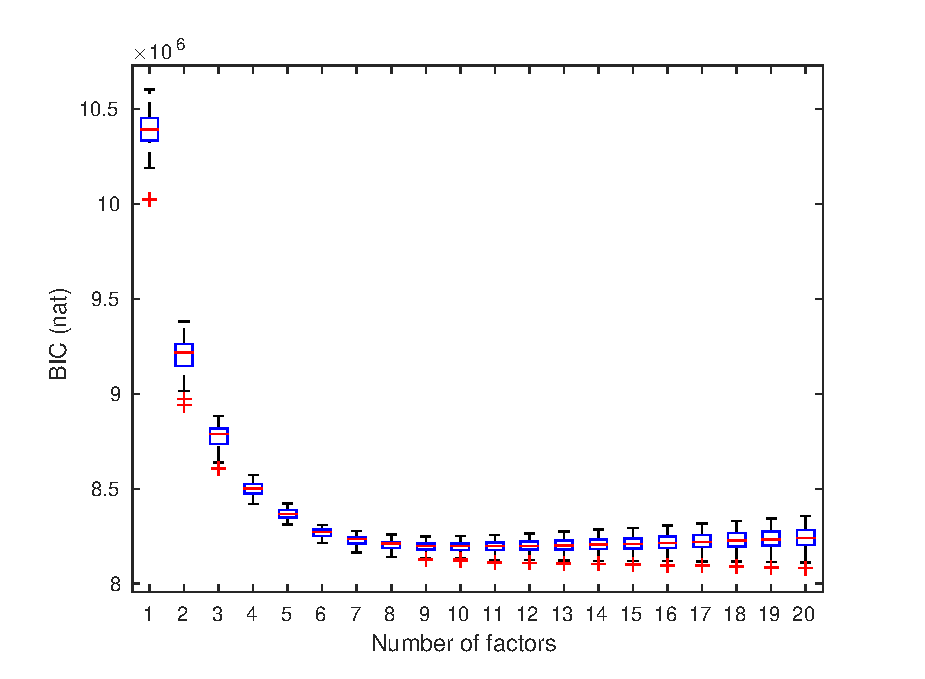
\includegraphics[width=0.75\textwidth]{figures/initial_factor_BIC_bootstrap.eps}
	\caption{BIC for fitting different number of factors onto the data. 99 bootstrap samples were used and only 1 initial value was used for each $k$. A stopping condition of 100 EM steps was used.}
	\label{fig:initial_factor_BIC_bootstrap}
\end{figure}

\section{Compound Poisson}
Consider photons emitted from an X-ray tube as a Poisson process. There has been Poisson latent models developed to consider such behaviour. For example the number of photons detected can be modelled as $Y\sim\poisson(\lambda)$ and then the grey value can be modelled as $X|Y\sim\normal(\alpha Y,\beta)$ \cite{jin2014investigating}. Such a model explains that there is a linear relationship between the mean and variance \cite{jin2014investigating}. However this does not consider that these photons have a board energy spectrum as a result of Bremsstrahlung and characteristic radiation. It can be shown that a compound Poisson model performs better \cite{whiting2006properties} because it considers the board energy spectrum of the photons. However fitting the model is very difficult using the EM algorithm and approximations have to be made \cite{xie2008x}.

\subsection{Theory}
Suppose an image has $m$ pixels and each pixel has a corresponding grey value $X_i$ for $i=1,2,\dotdotdot,m$. Let $Y_i$ be the number of photons detected in pixel $i$ and each photon has energy randomly distributed with mean $\mu_i$ and variance $\sigma_i^2$. The number of photons detected can be modelled as a Poisson process such that
\begin{equation}
Y_i\sim\poisson(\nu_i \tau)
\end{equation}
where $\nu_i$ is the post-attenuation rate and $\tau$ is the exposure time. The total amount of energy collected $U_i$ is then the sum of the energies of $Y_i$ photons. For large $Y_i$, the central limit theorem can be used so that $U_i$ is approximately Normally distributed so that
\begin{equation}
U_i|Y_i\sim\normal\left(
Y_i\mu_i,Y_i\sigma_i^2
\right) \ .
\end{equation}
Assuming the grey value is modelling the intensity, rate of energy per unit area, then $X_i$ can be modelled using
\begin{equation}
X_i|U_i\sim\normal\left(
\frac{\alpha}{\tau}U_i,\beta_i^2
\right)
\end{equation}
where $\alpha$ is some positive constant and $\beta_i^2$ is the variance of some additive normal noise.
 
The full joint probability density function is
\begin{equation*}
p_{X_i,U_i,Y_i}\left(x_i,u_i,y_i\right)=
p_{X_i|U_i}(x_i|u_i)p_{U_i|Y_i}(u_i|y_i)\prob(Y_i=y_i)
\end{equation*}
\begin{multline}
p_{X_i,U_i,Y_i}\left(x_i,u_i,y_i\right)=
\frac{1}{\sqrt{2\pi}\beta_i}\exp\left[-\frac{1}{2}\left(\frac{x_i-\alpha u_i /\tau}{\beta_i}\right)^2\right]
\\
\frac{1}{\sqrt{2\pi}\sqrt{y_i\sigma_i^2}}\exp\left[-\frac{1}{2}\left(\frac{u_i-y_i\mu_i}{\sqrt{y_i\sigma_i^2}}\right)^2\right]
\euler^{-\nu_i\tau}\frac{(\nu_i\tau)^{y_i}}{y_i!}
\end{multline}
for any real $x_i$, $u_i$ and $y_i=0,1,2,\dotdotdot$.
By marginalising out $U_i$, a one layer latent variable model can be obtained. Thus the EM algorithm \cite[pp.~260-261]{barber2012bayesian} can be used to estimate the unknown parameters $\nu_i,\mu_i,\sigma_i^2$ and $\beta_i^2$. The one layer latent variable is given as
\begin{equation}
Y_i\sim\poisson(\nu_i\tau)
\end{equation}
\begin{equation}
X_i|Y_i\sim\normal\left(
\frac{\alpha\mu_i}{\tau}Y_i,\frac{\alpha^2\sigma_i^2}{\tau^2}Y_i+\beta_i^2
\right) \ .
\end{equation}
The proof of this can be found in Appendix \ref{chapter:oneLayer_compoundPoisson}.

The marginal expectation and variance \cite[pp.~149-151]{rice2009mathematical} can be calculated
\begin{equation*}
\expectation[X_i]=\expectation[\expectation[X_i|Y_i]]
\end{equation*}
\begin{equation*}
\expectation[X_i]=\expectation\left[\frac{\alpha\mu_i}{\tau}Y_i\right]
\end{equation*}
\begin{equation}
\expectation[X_i] = \alpha \mu_i \nu_i
\end{equation}
and
\begin{equation*}
\variance[X_i] = \expectation[\variance[X_i|Y_i]] + \variance[\expectation[X_i|Y_i]]
\end{equation*}
\begin{equation*}
\variance[X_i] = \expectation\left[\frac{\alpha^2\sigma_i^2}{\tau^2}Y_i+\beta_i^2\right] + \variance\left[\frac{\alpha\mu_i}{\tau}Y_i\right]
\end{equation*}
\begin{equation*}
\variance[X_i] =
\frac{\alpha^2\sigma_i^2}{\tau^2}\nu_i\tau+\beta_i^2\
+\frac{\alpha^2\mu_i^2}{\tau^2}\nu_i\tau
\end{equation*}
\begin{equation}
\variance[X_i] = \frac{\alpha^2\nu_i}{\tau}\left(\mu_i^2+\sigma_i^2\right)+\beta_i^2 \ .
\end{equation}

This model can be made simpler by setting $\beta_i=0$ because by doing so the joint probability density function is in the exponential family with sufficient statistics $X_i^2/Y_i,X_i$ and $Y_i$. This is proven in Appendix \ref{chapter:compoundPoisson_expFamily}. However by doing so the joint probability density function must consider the special case of $Y_i=0$ because such a case will drive the variance of $X_i|Y_i$ to zero. This can be dealt with by using the Dirac delta function \cite[pp.~439-443]{riley2006mathematical}
\begin{equation*}
p_{X_i,Y_i}\left(x_i,y_i\right)=
p_{X_i|Y_i}(x_i|y_i)\prob(Y_i=y_i)
\end{equation*}
\begin{equation}
p_{X_i,Y_i}\left(x_i,y_i\right)=
\begin{cases}
\euler^{-\nu_i\tau}\delta(x) & \text{for }y=0
\\
\dfrac{\euler^{-\nu_i\tau}(\nu_i\tau)^{y_i}\tau}{y_i!\sqrt{2\pi y_i}\alpha\sigma_i}
\exp\left[-\dfrac{1}{2}\dfrac{\left(x_i-y_i\mu_i\alpha/\tau\right)^2}{\alpha^2y_i\sigma_i^2/\tau^2}\right] & \text{for }y=1,2,\dotdotdot
\end{cases} \ .
\end{equation}

The conditional probability mass function can be obtained by
\begin{equation*}
\prob\left(Y_i=y_i|X_i=x_i\right)=\frac{p_{X_i,Y_i}\left(x_i,y_i\right)}{p_{X_i}(x_i)}
\end{equation*}
where $p_{X_i}(x_i)$ is the normalization constant.
For the special cases
\begin{equation*}
\prob\left(Y_i=0|X_i=0\right) \propto \delta(0)
\end{equation*}
\begin{equation*}
\prob\left(Y_i=y|X_i=0\right) \propto
\dfrac{(\nu_i\tau)^{y_i}}{y_i!\sqrt{y_i}}
\exp\left[-\dfrac{1}{2}\dfrac{\left(x_i-y_i\mu_i\alpha/\tau\right)^2}{\alpha^2y_i\sigma_i^2/\tau^2}\right]
\quad \text{for }y=1,2,\dotdotdot \ .
\end{equation*}
But because $\delta(0)$ is infinite
\begin{equation}
\prob\left(Y_i=y|X_i=0\right) =
\begin{cases}
1 & \text{for }y=0
\\
0 & \text{for }y=1,2,\dotdotdot
\end{cases}
\end{equation}
and
\begin{equation}
\expectation[Y_i|X_i=0] = 0 \ .
\end{equation}
$\expectation[1/Y_i|X_i=0]$ cannot be defined in this special case.

Another special case is
\begin{equation*}
\prob\left(Y_i=0|X_i=x\right) \propto \delta(x) \quad \text{for }x\neq0
\end{equation*}
then
\begin{equation}
\prob\left(Y_i=0|X_i=x\right) = 0 \quad \text{for }x\neq0
\end{equation}

For the general case $y_i=1,2,\dotdotdot$ and $x_i\neq0$
\begin{equation}
\prob\left(Y_i=y_i|X_i=x_i\right)=\frac{1}{p_{X_i}(x_i)}\dfrac{\euler^{-\nu_i\tau}(\nu_i\tau)^{y_i}\tau}{y_i!\sqrt{2\pi y_i}\alpha\sigma_i}
\exp\left[-\dfrac{1}{2}\dfrac{\left(x_i-y_i\mu_i\alpha/\tau\right)^2}{\alpha^2y_i\sigma_i^2/\tau^2}\right]
\end{equation}
where
\begin{equation*}
p_{X_i}(x_i)=\sum_{y=0}^{\infty}p_{X_i,Y_i}(x_i,y_i)
\end{equation*}
\begin{equation}
p_{X_i}(x_i)=\sum_{y_i=1}^{\infty}\dfrac{\euler^{-\nu_i\tau}(\nu_i\tau)^{y_i}\tau}{y_i!\sqrt{2\pi y_i}\alpha\sigma_i}
\exp\left[-\dfrac{1}{2}\dfrac{\left(x_i-y_i\mu_i\alpha/\tau\right)^2}{\alpha^2y_i\sigma_i^2/\tau^2}\right] \ .
\end{equation}
The expectation of the sufficient statistics are then
\begin{equation}
\expectation\left[Y_i|X_i=x_i\right]=
\frac{1}{p_{X_i}(x_i)}
\sum_{y_i=1}^{\infty}\dfrac{\euler^{-\nu_i\tau}(\nu_i\tau)^{y_i}\tau}{y_i!\sqrt{2\pi}\alpha\sigma_i}y_i^{1/2}
\exp\left[-\dfrac{1}{2}\dfrac{\left(x_i-y_i\mu_i\alpha/\tau\right)^2}{\alpha^2y_i\sigma_i^2/\tau^2}\right]
\end{equation}
and
\begin{equation}
\expectation\left[\dfrac{1}{Y_i}|X_i=x_i\right]=
\frac{1}{p_{X_i}(x_i)}
\sum_{y_i=1}^{\infty}\dfrac{\euler^{-\nu_i\tau}(\nu_i\tau)^{y_i}\tau}{y_i!\sqrt{2\pi}\alpha\sigma_i}y_i^{-3/2}
\exp\left[-\dfrac{1}{2}\dfrac{\left(x_i-y_i\mu_i\alpha/\tau\right)^2}{\alpha^2y_i\sigma_i^2/\tau^2}\right] \ .
\end{equation}
Unfortunately such a sum cannot be simplified. The fastest approximate way to get a value for these expectations is to truncate the sum. Another way to obtain the conditional expectation is to use the sample mean from samples of the conditional distribution, however this could be slower depending on the sampling algorithm.

Because the conditional probability mass function is known up to a constant, rejection sampling can be used to draw conditional samples. Rejection sampling samples exactly but a proposal distribution is needed and this influences the rejection rate, or in other words the efficiency. One possible proposal is the Poisson distribution and there does exist adaptive methods which changes the proposal on the fly \cite{casella2004generalized}. Approximate Bayesian computation (ABC) \cite{marin2012approximate} can be used instead because $Y_i$ and $X_i|Y_i$ can be simulated. ABC draws approximate samples without a proposal but can suffer from high rejection rates.

Suppose for pixel $i$, the follow grey values have been observed $x_i^{(1)}$, $x_i^{(2)}$, $\dotdotdot$, $x_i^{(n)}$. For each corresponding observable let $Y_i^{(1)}$, $Y_i^{(2)}$, $\dotdotdot$, $Y_i^{(n)}$ be the Poisson latent variable. For the E step, $Y_i^{(j)}$ and $1/Y_i^{(j)}$ are estimated given all the parameters using the conditional expectation for $j=1,2,\dotdotdot,n$. That is $y_i^{(j)}=\expectation\left[Y_i^{(j)}|X_i^{(j)}=x_i^{(j)}\right]$ and $\zeta_i^{(j)}=\expectation\left[1/Y_i^{(j)}|X_i^{(j)}=x_i^{(j)}\right]$ respectively. 

In the M step the parameters $\nu_i,\mu_i,\sigma_i^2$ are estimated given the latent variables. This is done by maximising the conditional expectation of the log likelihood function, that is
\begin{equation}
H_i=\sum_{j=1}^n\expectation_{Y_i|X_i}\left[\ln p_{X_i,Y_i}\left(x_i^{(j)},Y_i^{(j)}\right)\right]
\end{equation}
It is given that the following M step estimators can be obtained:
\begin{equation}
\widehat{\mu}_i=\frac{\tau\sum_{j=1}^nx_i^{(j)}}{\alpha\sum_{j=1}^ny_i^{(j)}}
\end{equation}
\begin{equation}
\widehat{\sigma}_i^2=\frac{1}{n}\left[
\frac{\tau^2}{\alpha^2}\sum_{j=1}^n\left(x_i^{(j)}\right)^2\zeta_i^{(j)}
-\frac{2\tau\mu_i}{\alpha}\sum_{j=1}^nx_i^{(j)}
+\mu_i^2\sum_{j=1}^ny_i^{(j)}
\right]
\end{equation}
\begin{equation}
\widehat{\nu}_i=\frac{\sum_{j=1}^ny_i^{(j)}}{n\tau}
\end{equation}
where $\left(x_i^{(j)}\right)^2\zeta_i^{(j)}=0$ if $\left(x_i^{(j)}\right)^2=0$. This is proven in Appendix \ref{chapter:mStep_compoundPoisson}.

The constant $\alpha$ only sets the scale of $\mu_i$ and $\sigma_i^2$ but can be calibrated so that it has units of keV. From Chapter \ref{chapter:about_the_data}, the following properties of the X-ray tube were stated or calculated:
\begin{itemize}
	\item Voltage = $V$ = 100 kV
	\item Power = $P$ = 33.0 W
	\item Exposure time = $\tau$ = 500 ms
	\item Efficiency = $\eta = 8.1\times10^{-3}$
	\item Target material is tungsten.
\end{itemize}
Assume, very crudely, the X-ray spreads out and targets the detector with $1996^2$ pixels only and nothing else, then the total energy detected in one pixel is
\begin{equation}
U=\frac{\eta P\tau}{1996^2}=2.1\times10^{8}\text{ keV}\cdot\text{pixel}^{-1} \ .
\end{equation}
The images were calibrated so that the background has grey value of 60\,000. Assuming the air has attenuation coefficient of zero, then $\alpha$ can be estimated by
\begin{equation}
\alpha = \frac{60\,000 \tau}{U} = 1.4\times10^{-4}\text{ s}\cdot\text{keV}^{-1}\cdot\text{pixel} \ .
\end{equation}
This calculation could be improved if the solid angle of the X-ray beam and the distance between the X-ray tube and X-ray detector were given.

\subsection{Toy Example}
A dataset was simulated, with $n=100$ samples, using the follow parameters with arbitrary units: $\alpha=1$, $\tau=1$, $\nu=5$, $\mu=3$ and $\sigma^2=0.1$. The EM algorithm was initialized by assigning each latent variable such that $Y^{(j)}\sim\poisson(\phi)$ for i.i.d.~$j=1,2,\dotdotdot,n$. The sums, to work out the expectations and likelihood, were truncated to include 100 terms.

The figures showed that the EM algorithm works because for different initial values, the parameters converge towards the true value and the log likelihood always increases.

For high $\nu\tau$, problems arises as more and more terms are needed in the truncated sum. Too many terms in the truncated sum slow down the program a lot.

\begin{figure}
	\centering
	\begin{subfigure}{0.45\textwidth}
		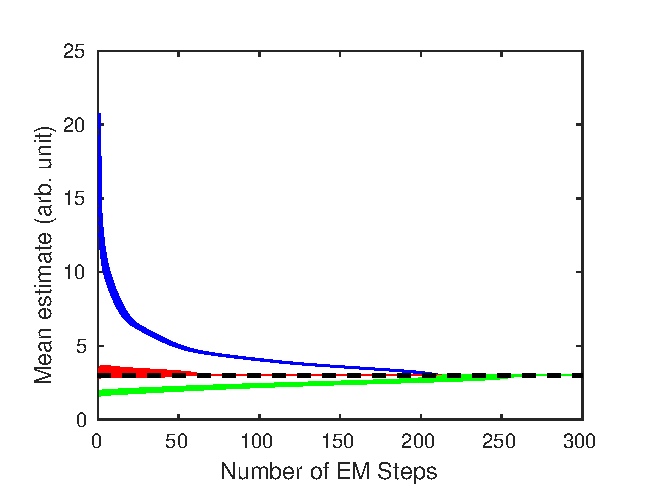
\includegraphics[width=\textwidth]{figures/hierarchicalModel/EM_initial_mean.eps}
	\end{subfigure}
	\begin{subfigure}{0.45\textwidth}
		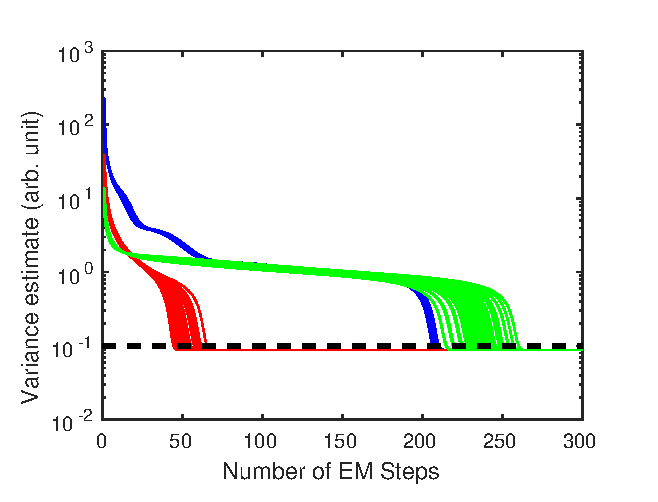
\includegraphics[width=\textwidth]{figures/hierarchicalModel/EM_initial_var.eps}
	\end{subfigure}
	\begin{subfigure}{0.45\textwidth}
		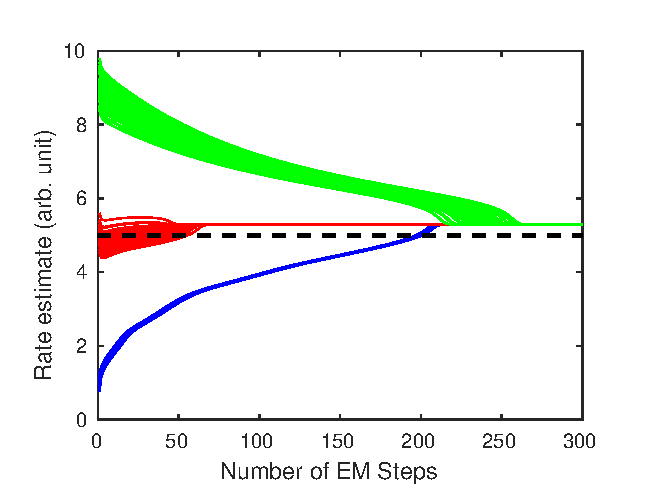
\includegraphics[width=\textwidth]{figures/hierarchicalModel/EM_initial_rate.eps}
	\end{subfigure}
	\begin{subfigure}{0.45\textwidth}
		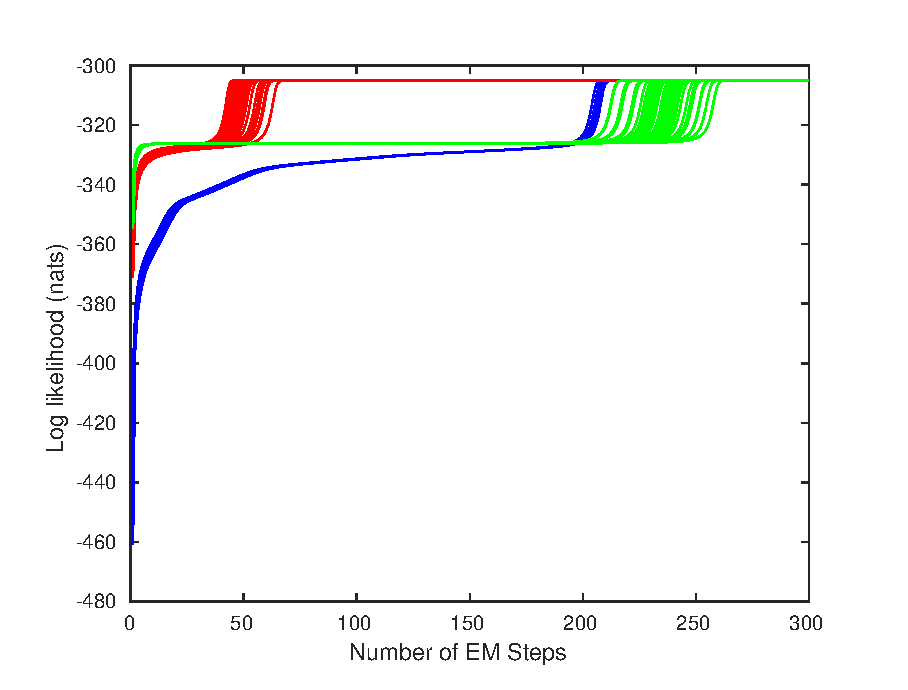
\includegraphics[width=\textwidth]{figures/hierarchicalModel/EM_initial_lnL.eps}
	\end{subfigure}
	\caption{The parameters and log likelihood at each step of EM. The EM algorithm was used to estimate the parameters of a single simulated $n=100$ dataset. The latent variables were initialized $\poisson(\phi)$ 50 times. Blue: $\phi=1$, Red: $\phi=4$, Green: $\phi=9$. Dotted line: true value}
\end{figure}

\begin{figure}
	\centering
	\begin{subfigure}{0.45\textwidth}
		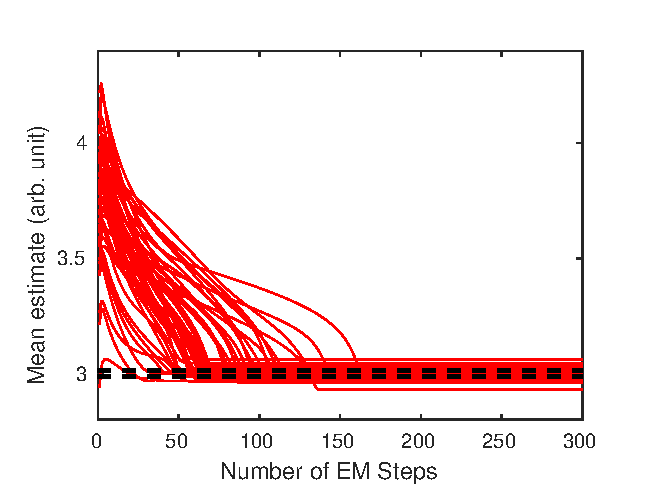
\includegraphics[width=\textwidth]{figures/hierarchicalModel/EM_repeat_mean.eps}
	\end{subfigure}
	\begin{subfigure}{0.45\textwidth}
		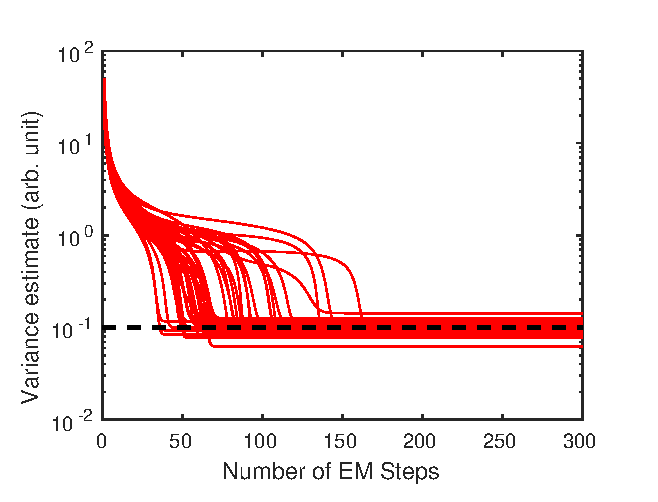
\includegraphics[width=\textwidth]{figures/hierarchicalModel/EM_repeat_variance.eps}
	\end{subfigure}
	\begin{subfigure}{0.45\textwidth}
		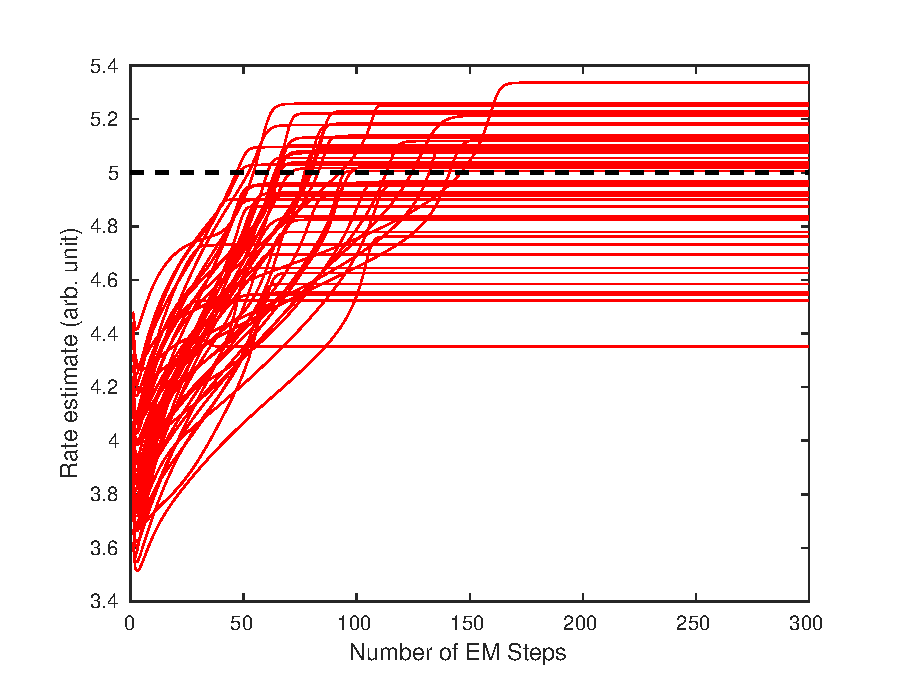
\includegraphics[width=\textwidth]{figures/hierarchicalModel/EM_repeat_rate.eps}
	\end{subfigure}
	\begin{subfigure}{0.45\textwidth}
		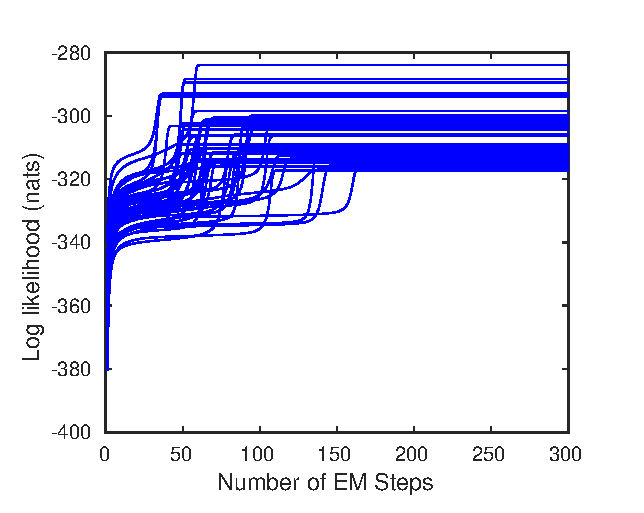
\includegraphics[width=\textwidth]{figures/hierarchicalModel/EM_repeat_lnL.eps}
	\end{subfigure}
	\caption{The parameters and log likelihood at each step of EM. The EM algorithm was used to estimate the parameters of 50 different simulated $n=100$ dataset. The latent variables were initialized $\poisson(4)$. Dotted line: true value}
\end{figure}

%=======CONCLUSION===============
\chapter{Conclusion}

\section{Mean and Variance Relationship}
The relationship between the sample mean and sample variance of the grey values was modelled by fitting a weighted linear regression. Less weights were given to bigger sample variance as a simple method for robust regression. It was found that the mean and variance relationship depended on the different materials: the 3D printed sample, the background and the foam holder. To take into account the different mean and variance relationships, a mixture of linear regression was fitted but it failed to capture the different behaviours from the different materials. Weighted linear regression, where the weights depended on the difference between the sample mean grey value and some $k$ mean sample mean grey value, was fitted and only captured 2 out of the 3 material mean variance relationship.

There is further work to do in the mean and variance relationship. Firstly it should be investigated whenever transforming the variance will produce a more linear model. For example the log variance or the standard deviation could be used. Furthermore, more features than just polynomials should be used for the sample mean grey values. Lastly, it was established that the sample variance has a scaled $\chi^2$ distribution. Because the $\chi^2$ distribution is in the exponential family, generalised linear models \cite{mccullagh1989generalized} should be used as well to open up more possibilities to model the relationship between the mean and variance.

\section{Latent Variable Model}
In order to be able to find sources of variance, latent variable models were used as a way to develop explanatory models. PCA and factor analysis were used on a shrunken down dataset and found the 3D printed sample does have a lower sample variance. It was also found that the background variance was not uniform and there are patches of high variance. However shrinking the images down could be a problem because this could of affected the variance of the dataset. In order to improve the data analysis, the computational algorithms should be improved so that PCA and factor analysis can be done directly on the full size dataset.

Another explanatory model developed under the light of physics was the compound Poisson distribution. While the compound Poisson distribution was used in the medical physics community \cite{whiting2006properties}, fitting the distribution was extremely difficult because conditional and marginal distribution cannot be written down in closed form. A toy example was provided in this report. In order for the fitting to work computationally, approximations which are cheap to run must be made.

\appendix

\chapter{Source Code}

\chapter{Proofs and Identities}

\section{Matrix Calculus}\label{chapter:matrixCalculus}
Let $\matr{A},\matr{B},\matr{C}$ be matrices with elements
\begin{equation*}
\matr{A}=
\begin{pmatrix}
a_{1,1}&a_{1,2}&\cdots&a_{1,n} \\
a_{2,1}&a_{2,2}&\cdots&a_{2,n} \\
\vdots&\vdots&\ddots&\vdots \\
a_{m,1}&a_{m,2}&\cdots&a_{m,n} 
\end{pmatrix}
\end{equation*}
and similar for $\matr{B}$ and $\matr{C}$.

Let $\matr{D_{A}}$ be the gradient operator such that
\begin{equation*}
\matr{D_{A}}=
\begin{pmatrix}
\partial/\partial a_{1,1}&\partial/\partial a_{1,2}&\cdots&\partial/\partial a_{1,n} \\
\partial/\partial a_{2,1}&\partial/\partial a_{2,2}&\cdots&\partial/\partial a_{2,n} \\
\vdots&\vdots&\ddots&\vdots \\
\partial/\partial a_{m,1}&\partial/\partial a_{m,2}&\cdots&\partial/\partial a_{m,n} 
\end{pmatrix}
\end{equation*}
then it can be shown that \cite{petersen2008matrix}
\begin{equation}
\matr{D_{A}}\trace\left(\matr{A}\T\matr{B}\right) = \matr{B}
\end{equation}
\begin{equation}
\matr{D_{A}}\trace\left(\matr{A}\T\matr{B}\matr{A}\matr{C}\right) = \matr{B}\matr{A}\matr{C}+\matr{B}\T\matr{A}\matr{C}\T
\end{equation}
\begin{equation}
\matr{D_{A}}\ln\left\|\matr{A}\right\| = \left(\matr{A}^{-1}\right)\T \ .
\end{equation}
Because a vector is a special case of a matrix, these results can be extended to vectors.


\section{M Step for Mixture of Linear Regression} \label{section:Mstep}
The likelihood for a general mixture model is
\begin{equation*}
\ln{L}=\sum_{i=1}^m\ln\left[
\sum_{j=1}^qp_{Y|S}\left(y_i|S_i=j\right)\pi_j
\right]
\end{equation*}
In the M step, the parameters $\vectGreek{\beta}_j$, $\sigma_j^2$ and $\pi_j$ for $j=1,2,\dotdotdot,q$ are updated given the posterior distribution of $S_i$ for $i=1,2,\dotdotdot,m$. Consider some arbitrary parameter $\theta_j$ which model $j$ depends on. Then
\begin{equation*}
\frac{\partial\ln{L}}{\partial\theta_j}=
\sum_{i=1}^m\frac{\pi_j}{\sum_{j'=1}^qp_{Y|S}\left(y_i|S_i=j'\right)\pi_j}
\frac{\partial p_{Y|S}\left(y_i|S_i=j\right)}{\partial\theta_j}
\end{equation*}
\begin{equation*}
\frac{\partial\ln{L}}{\partial\theta_j}=
\sum_{i=1}^m\frac{p_{Y|S}\left(y_i|S_i=j\right)\pi_j}{\sum_{j'=1}^qp_{Y|S}\left(y_i|S_i=j'\right)\pi_j}
\frac{\partial \ln\left[p_{Y|S}\left(y_i|S_i=j\right)\right]}{\partial\theta_j}
\end{equation*}
which is just
\begin{equation}
\frac{\partial\ln{L}}{\partial\theta_j}=
\sum_{i=1}^mr_{i,j}
\frac{\partial \ln\left[p_{Y|S}\left(y_i|S_i=j\right)\right]}{\partial\theta_j} \ .
\end{equation}
Using the above result
\begin{equation*}
\nabla_{\vectGreek{\beta}_j}\ln{L}
=\sum_{i=1}^{m}
r_{i,j}
\nabla_{\vectGreek{\beta}_j}
\ln\left[
	\frac{1}{\sqrt{2\pi}\sigma_j}\exp\left(-\frac{1}{2}\left(\frac{y_i-\left(\vect{x}_i\right)\T\vectGreek{\beta}_j}{\sigma_j}\right)^2\right)
\right]
\end{equation*}
\begin{equation*}
\nabla_{\vectGreek{\beta}_j}\ln{L}
=\sum_{i=1}^{m}
r_{i,j}
\nabla_{\vectGreek{\beta}_j}
\left[
	-\frac{1}{2}\ln(2\pi) - \frac{1}{2}\ln\left(\sigma_j^2\right)-\frac{1}{2}\left(\frac{y_i-\left(\vect{x}_i\right)\T\vectGreek{\beta}_j}{\sigma_j}\right)^2
\right] \ .
\end{equation*}
Expanding it out
\begin{equation*}
\nabla_{\vectGreek{\beta}_j}\ln{L}
=\sum_{i=1}^{m}
r_{i,j}
\nabla_{\vectGreek{\beta}_j}
\left[-\frac{1}{2\sigma_j^2}\left(-2y_i\vectGreek{\beta}_j\T\vect{x}_i
+\vectGreek{\beta}_j\T\vect{x}_i\left(\vect{x}_i\right)\T\vectGreek{\beta}_j
\right)
+c_1
\right]
\end{equation*}
and using the properties of the trace
\begin{equation*}
\nabla_{\vectGreek{\beta}_j}\ln{L}
=\sum_{i=1}^{m}
r_{i,j}
\nabla_{\vectGreek{\beta}_j}
\left[-\frac{1}{2\sigma_j^2}\left(-2y_i\trace\left(\vectGreek{\beta}_j\T\vect{x}_i\right)
+\trace\left(\vectGreek{\beta}_j\T\vect{x}_i\left(\vect{x}_i\right)\T\vectGreek{\beta}_j
\right)\right)
+c_1
\right]
\end{equation*}
together with the results in Appendix \ref{chapter:matrixCalculus}
\begin{equation}
\nabla_{\vectGreek{\beta}_j}\ln{L}
=\sum_{i=1}^{m}
-\frac{r_{i,j}}{2\sigma_j^2}
\left(-2y_i\vect{x}_i
+2\vect{x}_i\left(\vect{x}_i\right)\T\vectGreek{\beta}_j
\right) \ .
\end{equation}
Setting this to zero
\begin{equation*}
\sum_{i=1}^{m}
r_{i,j}
y_i\vect{x}_i
=
\sum_{i=1}^{m}r_{i,j}
\vect{x}_i\left(\vect{x}_i\right)\T\widehat{\vectGreek{\beta}}_j
\end{equation*}
\begin{equation}
\widehat{\vectGreek{\beta}}_j
=
\left[\sum_{i=1}^{m}r_{i,j}
\vect{x}_i\left(\vect{x}_i\right)\T\right]^{-1}
\left[\sum_{i=1}^{m}
r_{i,j}
y_i\vect{x}_i\right]
\end{equation}
and this is just weighted least squares where the weights are the responsibilities on model $j$.

By re-parametrise $1/\sigma_j^2=\tau_j$
\begin{equation*}
\frac{\partial\ln{L}}{\partial\tau_j}
=\sum_{i=1}^{m}
r_{i,j}
\frac{\partial}{\partial\tau_j}
\left[
	-\frac{1}{2}\ln(2\pi) + \frac{1}{2}\ln\left(\tau_j\right)-\frac{\tau_j}{2}\left({y_i-\left(\vect{x}_i\right)\T\vectGreek{\beta}_j}\right)^2
\right]
\end{equation*}
\begin{equation}
\frac{\partial\ln{L}}{\partial\tau_j}
=\sum_{i=1}^{m}
r_{i,j}
\left[\frac{1}{2\tau_j}-\frac{1}{2}\left({y_i-\left(\vect{x}_i\right)\T\vectGreek{\beta}_j}\right)^2
\right] \ .
\end{equation}
Setting this to zero
\begin{equation}
\widehat{\sigma}_j^2
=
\frac{\sum_{i=1}^{m}
r_{i,j}\left({y_i-\left(\vect{x}_i\right)\T\vectGreek{\beta}_j}\right)^2}
{\sum_{i=1}^{m}r_{i,j}}
\end{equation}
and this is the weighted mean squared error.

To obtain the maximum log likelihood estimator for $\pi_j$, a Lagrange multiplier must be used to put a constraint that $\sum_{j=1}^q\pi_j=1$. The objective is then
\begin{equation*}
T = \ln{L} + \lambda\left(\sum_{j=1}^q\pi_j-1\right)
\end{equation*}
\begin{equation*}
\frac{\partial T}{\partial\pi_j}=\frac{\partial}{\partial\pi_j}\sum_{i=1}^m\ln\left[
\sum_{j'=1}^qp_{Y|S}\left(y_i|S_i=j'\right)\pi_{j'}
\right] + \lambda
\end{equation*}
\begin{equation*}
\frac{\partial T}{\partial\pi_j}=\sum_{i=1}^m\frac{p_{Y|S}\left(y_i|S_i=j\right)}{\sum_{j'=1}^qp_{Y|S}\left(y_i|S_i=j'\right)\pi_{j'}} + \lambda
\end{equation*}
\begin{equation}
\frac{\partial T}{\partial\pi_j}=\sum_{i=1}^m\frac{r_{i,j}}{\pi_j} + \lambda \ .
\end{equation}
Setting this to zero
\begin{equation}
\widehat{\pi}_j = \sum_{i=1}^m\frac{r_{i,j}}{\lambda} \ .
\end{equation}
$\lambda$ can be determined by putting a constraint on the estimators of $\pi_j$ for $j=1,2,\dotdotdot,q$
\begin{equation*}
\sum_{j=1}^q\sum_{i=1}^m\frac{r_{i,j}}{\lambda}=1
\end{equation*}
\begin{equation*}
\sum_{i=1}^m\sum_{j=1}^qr_{i,j}=\lambda
\end{equation*}
\begin{equation*}
\sum_{i=1}^m1=\lambda
\end{equation*}
\begin{equation}
m=\lambda
\end{equation}
therefore
\begin{equation}
\widehat{\pi}_j = \sum_{i=1}^m\frac{r_{i,j}}{m} \ .
\end{equation}
This is the average responsibility.

\section{M Step for Factor Analysis}\label{chapter:mStep_factorAnalysis}
The objective is to maximise is the condition expectation of the log joint likelihood, that is
\begin{equation*}
H = \expectation_{\vect{Y}|\vect{X}}\left[\sum_{i=1}^{n}\ln p_{\vect{X},\vect{Y}}\left(\vect{x}^{(i)},\vect{Y}^{(i)}\right)\right] \ .
\end{equation*}
This can be expressed as
\begin{equation*}
H = \expectation_{\vect{Y}|\vect{X}}\left[
\sum_{i=1}^{n}\left(\ln p_{\vect{X}|\vect{Y}}\left(\vect{x}^{(i)}|\vect{Y}^{(i)}\right)+\ln p_{\vect{Y}}\left(\vect{Y}^{(i)}\right)\right)
\right]
\end{equation*}
Because the marginal distribution of the latent variables do not depend on $\matr{\Lambda}$ and $\matr{\Psi}$, the last term can be ignored. Using Equation \eqref{eq:factor_analysis_x_given_y_dist}
\begin{multline*}
H = \expectation_{\vect{Y}|\vect{X}}\left[
\sum_{i=1}^{n}\ln\left(\frac{1}{\|2\pi\matr{\Psi}\|^{1/2}}
\right.\right.
\\
\left.\left.
\exp\left(-\frac{1}{2}\left(\vect{x}^{(i)}-\matr{\Lambda}\vect{Y}^{(i)}\right)\T\matr{\Psi}^{-1}\left(\vect{x}^{(i)}-\matr{\Lambda}\vect{Y}^{(i)}\right)\right)\right)
\right]
+c_1
\end{multline*}
\begin{multline*}
H = \expectation_{\vect{Y}|\vect{X}}\left[
\sum_{i=1}^{n}\left(-\frac{1}{2}\ln{\|2\pi\matr{\Psi}\|}
\right.\right.
\\
\left.\left.
-\frac{1}{2}\left(\vect{x}^{(i)}-\matr{\Lambda}\vect{Y}^{(i)}\right)\T\matr{\Psi}^{-1}\left(\vect{x}^{(i)}-\matr{\Lambda}\vect{Y}^{(i)}\right)\right)
\right]
+c_1
\end{multline*}
\begin{multline*}
H = -\frac{1}{2}\expectation_{\vect{Y}|\vect{X}}\left[
\sum_{i=1}^{n}\left(\ln{\|2\pi\matr{\Psi}\|}+\left(\vect{x}^{(i)}\right)\T\matr{\Psi}^{-1}\matr{\Lambda}\vect{Y}^{(i)}
\right.\right.
\\
\left.\left.
-2\left(\vect{x}^{(i)}\right)\T\matr{\Psi}^{-1}\matr{\Lambda}\vect{Y}^{(i)}+\left(\vect{Y}^{(i)}\right)\T\matr{\Lambda}\T\matr{\Psi}^{-1}\matr{\Lambda}\vect{Y}^{(i)}\right)
\right]
+c_1
\end{multline*}
By defining
\begin{equation}
\expectation_{\vect{Y}|\vect{X}}\left[\vect{Y}^{(i)}|\vect{X}^{(i)}=\vect{x}^{(i)}\right]=\vect{y}^{(i)}
\end{equation}
and
\begin{equation}
\cov\left[\vect{Y}^{(i)}|\vect{X}^{(i)}=\vect{x}^{(i)}\right] = \matr{\Sigma}_{\vect{Y}}
\end{equation}
then when taking the conditional expectation
\begin{multline*}
H = -\frac{1}{2}\sum_{i=1}^{n}\left[
\ln\|2\pi\matr{\Psi}\|+\left(\vect{x}^{(i)}\right)\T\matr{\Psi}^{-1}\vect{x}^{(i)}-2\left(\vect{x}^{(i)}\right)\T\matr{\Psi}^{-1}\matr{\Lambda}\vect{y}^{(i)}\right.\\
\left.+\trace\left(\matr{\Lambda}\T\matr{\Psi}^{-1}\matr{\Lambda}\matr{\Sigma}_{\vect{Y}}\right)+\left(\vect{y}^{(i)}\right)\T\matr{\Lambda}\T\matr{\Psi}^{-1}\matr{\Lambda}\vect{y}^{(i)}
\right]+c_1
\end{multline*}
\begin{multline*}
H = -\frac{1}{2}\sum_{i=1}^{n}\left[
\ln\|2\pi\matr{\Psi}\|+\left(\vect{x}^{(i)}\right)\T\matr{\Psi}^{-1}\vect{x}^{(i)}-2\left(\vect{x}^{(i)}\right)\T\matr{\Psi}^{-1}\matr{\Lambda}\vect{y}^{(i)}\right.\\
\left.+\trace\left(\matr{\Lambda}\T\matr{\Psi}^{-1}\matr{\Lambda}\matr{\Sigma}_{\vect{Y}}\right)+\trace\left(\matr{\Lambda}\T\matr{\Psi}^{-1}\matr{\Lambda}\vect{y}^{(i)}\left(\vect{y}^{(i)}\right)\T\right)
\right]+c_1
\end{multline*}
\begin{multline*}
H = -\frac{1}{2}\sum_{i=1}^{n}\left[
\ln\|2\pi\matr{\Psi}\|+\left(\vect{x}^{(i)}\right)\T\matr{\Psi}^{-1}\vect{x}^{(i)}-2\left(\vect{x}^{(i)}\right)\T\matr{\Psi}^{-1}\matr{\Lambda}\vect{y}^{(i)}\right.\\
\left.+\trace\left(\matr{\Lambda}\T\matr{\Psi}^{-1}\matr{\Lambda}\left(\matr{\Sigma}_{\vect{Y}}+\vect{y}^{(i)}\left(\vect{y}^{(i)}\right)\T\right)\right)
\right]+c_1
\end{multline*}
\begin{multline*}
H = -\frac{n}{2}
\ln\|\matr{\Psi}\|
-\frac{1}{2}\sum_{i=1}^{n}\left(\vect{x}^{(i)}\right)\T\matr{\Psi}^{-1}\vect{x}^{(i)}
+\sum_{i=1}^{n}\left(\vect{x}^{(i)}\right)\T\matr{\Psi}^{-1}\matr{\Lambda}\vect{y}^{(i)}\\
-\frac{1}{2}\sum_{i=1}^{n}\trace\left(\matr{\Lambda}\T\matr{\Psi}^{-1}\matr{\Lambda}\left(\matr{\Sigma}_{\vect{Y}}+\vect{y}^{(i)}\left(\vect{y}^{(i)}\right)\T\right)\right)
+c_2
\end{multline*}

Taking the derivative with respect to $\matr{\Lambda}$
\begin{equation*}
\matr{D}_{\matr{\Lambda}}H=
\matr{D}_{\matr{\Lambda}}\left[
\sum_{i=1}^n\left(\vect{x}^{(i)}\right)\T\matr{\Psi}^{-1}\matr{\Lambda}\vect{y}^{(i)}
-\frac{1}{2}\sum_{i=1}^{n}\trace\left(\matr{\Lambda}\T\matr{\Psi}^{-1}\matr{\Lambda}\left(\matr{\Sigma}_{\vect{Y}}+\vect{y}^{(i)}\left(\vect{y}^{(i)}\right)\T\right)\right)
\right]
\end{equation*}
\begin{multline*}
\matr{D}_{\matr{\Lambda}}H=
\matr{D}_{\matr{\Lambda}}\left[
\sum_{i=1}^n\trace\left(\left(\vect{y}^{(i)}\right)\T\matr{\Lambda}\T\matr{\Psi}^{-1}\vect{x}^{(i)}\right)
\right.
\\
\left.
-\frac{1}{2}\sum_{i=1}^{n}\trace\left(\matr{\Lambda}\T\matr{\Psi}^{-1}\matr{\Lambda}\left(\matr{\Sigma}_{\vect{Y}}+\vect{y}^{(i)}\left(\vect{y}^{(i)}\right)\T\right)\right)
\right]
\end{multline*}
\begin{multline*}
\matr{D}_{\matr{\Lambda}}H=
\matr{D}_{\matr{\Lambda}}\left[
\sum_{i=1}^n\trace\left(\matr{\Lambda}\T\matr{\Psi}^{-1}\vect{x}^{(i)}\left(\vect{y}^{(i)}\right)\T\right)
\right.
\\
\left.
-\frac{1}{2}\sum_{i=1}^{n}\trace\left(\matr{\Lambda}\T\matr{\Psi}^{-1}\matr{\Lambda}\left(\matr{\Sigma}_{\vect{Y}}+\vect{y}^{(i)}\left(\vect{y}^{(i)}\right)\T\right)\right)
\right]
\end{multline*}
\begin{equation*}
\matr{D}_{\matr{\Lambda}}H=
\sum_{i=1}^n\matr{\Psi}^{-1}\vect{x}^{(i)}\left(\vect{y}^{(i)}\right)\T
-\sum_{i=1}^{n}\matr{\Psi}^{-1}\matr{\Lambda}\left(\matr{\Sigma}_{\vect{Y}}+\vect{y}^{(i)}\left(\vect{y}^{(i)}\right)\T\right) \ .
\end{equation*}
Setting the derivative to zero
\begin{equation*}
\matr{0}=
\sum_{i=1}^n\matr{\Psi}^{-1}\vect{x}^{(i)}\left(\vect{y}^{(i)}\right)\T
-\sum_{i=1}^{n}\matr{\Psi}^{-1}\matr{\Lambda}\left(\matr{\Sigma}_{\vect{Y}}+\vect{y}^{(i)}\left(\vect{y}^{(i)}\right)\T\right) \ .
\end{equation*}
\begin{equation*}
\matr{0}=
\sum_{i=1}^n\vect{x}^{(i)}\left(\vect{y}^{(i)}\right)\T
-\matr{\Lambda}\left(n\matr{\Sigma}_{\vect{Y}}+\sum_{i=1}^{n}\vect{y}^{(i)}\left(\vect{y}^{(i)}\right)\T\right)
\end{equation*}
\begin{equation}
\matr{\Lambda}
=
\left(\sum_{i=1}^n\vect{x}^{(i)}\left(\vect{y}^{(i)}\right)\T\right)\left(n\matr{\Sigma}_{\vect{Y}}+\sum_{i=1}^{n}\vect{y}^{(i)}\left(\vect{y}^{(i)}\right)\T\right)^{-1}\ .
\end{equation}

The objective can be re-parametrised using $\matr{T}=\matr{\Psi}^{-1}$ so that
\begin{multline*}
H = -\frac{n}{2}
\ln\|\matr{T^{-1}}\|
-\frac{1}{2}\sum_{i=1}^{n}\left(\vect{x}^{(i)}\right)\T\matr{T}\vect{x}^{(i)}
+\sum_{i=1}^{n}\left(\vect{x}^{(i)}\right)\T\matr{T}\matr{\Lambda}\vect{y}^{(i)}\\
-\frac{1}{2}\sum_{i=1}^{n}\trace\left(\matr{\Lambda}\T\matr{T}\matr{\Lambda}\left(\matr{\Sigma}_{\vect{Y}}+\vect{y}^{(i)}\left(\vect{y}^{(i)}\right)\T\right)\right)
+c_2
\end{multline*}
\begin{multline*}
H = -\frac{n}{2}
\ln\|\matr{T^{-1}}\|
-\frac{1}{2}\sum_{i=1}^{n}\left(\vect{x}^{(i)}\right)\T\matr{T}\vect{x}^{(i)}
+\sum_{i=1}^{n}\left(\vect{x}^{(i)}\right)\T\matr{T}\matr{\Lambda}\vect{y}^{(i)}\\
-\frac{1}{2}\sum_{i=1}^{n}\trace\left(\matr{\Lambda}\T\matr{T}\matr{\Lambda}\left(\matr{\Sigma}_{\vect{Y}}+\vect{y}^{(i)}\left(\vect{y}^{(i)}\right)\T\right)\right)
+c_2 \ .
\end{multline*}
$\|\matr{T}^{-1}\| = 1/\|\matr{T}\|$ and using the properties of the trace
\begin{multline*}
H = \frac{n}{2}
\ln\|\matr{T}\|
-\frac{1}{2}\sum_{i=1}^{n}\trace\left(\matr{T}\vect{x}^{(i)}\left(\vect{x}^{(i)}\right)\T\right)
+\sum_{i=1}^{n}\trace\left(\matr{T}\matr{\Lambda}\vect{y}^{(i)}\left(\vect{x}^{(i)}\right)\T\right)\\
-\sum_{i=1}^{n}\frac{1}{2}\trace\left(\matr{T}\matr{\Lambda}\left(\matr{\Sigma}_{\vect{Y}}+\vect{y}^{(i)}\left(\vect{y}^{(i)}\right)\T\right)\matr{\Lambda}\T\right)
+c_2 \ .
\end{multline*}
Taking the derivative with respect to $\matr{\Psi}$
\begin{multline*}
\matr{D}_{\matr{\Psi}}H = \frac{n}{2}\matr{T}^{-1}
-\frac{1}{2}\sum_{i=1}^{n}\vect{x}^{(i)}\left(\vect{x}^{(i)}\right)\T
+\sum_{i=1}^{n}\matr{\Lambda}\vect{y}^{(i)}\left(\vect{x}^{(i)}\right)\T\\
-\sum_{i=1}^{n}\frac{1}{2}\matr{\Lambda}\left(\matr{\Sigma}_{\vect{Y}}+\vect{y}^{(i)}\left(\vect{y}^{(i)}\right)\T\right)\matr{\Lambda}\T \ .
\end{multline*}
Setting the derivative to zero
\begin{multline*}
\matr{0} = \frac{n}{2}\matr{\Psi}
-\frac{1}{2}\sum_{i=1}^{n}\vect{x}^{(i)}\left(\vect{x}^{(i)}\right)\T
+\sum_{i=1}^{n}\matr{\Lambda}\vect{y}^{(i)}\left(\vect{x}^{(i)}\right)\T\\
-\frac{n}{2}\matr{\Lambda}\matr{\Sigma}_{\vect{Y}}\matr{\Lambda}-\frac{1}{2}\matr{\Lambda}\sum_{i=1}^{n}\vect{y}^{(i)}\left(\vect{y}^{(i)}\right)\T)\matr{\Lambda}\T
\end{multline*}
\begin{equation*}
\matr{0} = \frac{n}{2}\matr{\Psi}
-\frac{1}{2}\sum_{i=1}^{n}\left(
\left(\vect{x}^{(i)}-\matr{\Lambda}\vect{y}^{(i)}\right)
\left(\vect{x}^{(i)}-\matr{\Lambda}\vect{y}^{(i)}\right)\T
\right)
-\frac{n}{2}\matr{\Lambda}\matr{\Sigma}_{\vect{Y}}\matr{\Lambda}
\end{equation*}
\begin{equation}
\matr{\Psi} =
\frac{1}{n}\sum_{i=1}^{n}\left(
\left(\vect{x}^{(i)}-\matr{\Lambda}\vect{y}^{(i)}\right)
\left(\vect{x}^{(i)}-\matr{\Lambda}\vect{y}^{(i)}\right)\T
\right)
+\matr{\Lambda}\matr{\Sigma}_{\vect{Y}}\matr{\Lambda}\ .
\end{equation}
Because $\matr{\Psi}$ is a diagonal matrix, only the diagonal entries need to be updated.

\section{Obtaining a One-Layer Compound Poisson Model}\label{chapter:oneLayer_compoundPoisson}
The full joint probability density function is
\begin{equation*}
p_{X_i,U_i,Y_i}\left(x_i,u_i,y_i\right)=
p_{X_i|U_i}(x_i|u_i)p_{U_i|Y_i}(u_i|y_i)\prob(Y_i=y_i)
\end{equation*}
\begin{multline}
p_{X_i,U_i,Y_i}\left(x_i,u_i,y_i\right)=
\frac{1}{\sqrt{2\pi}\beta_i}\exp\left[-\frac{1}{2}\left(\frac{x_i-\alpha u_i /\tau}{\beta_i}\right)^2\right]
\\
\frac{1}{\sqrt{2\pi}\sqrt{y_i\sigma_i^2}}\exp\left[-\frac{1}{2}\left(\frac{u_i-y_i\mu_i}{\sqrt{y_i\sigma_i^2}}\right)^2\right]
\euler^{-\nu_i\tau}\frac{(\nu_i\tau)^{y_i}}{y_i!} \ .
\end{multline}

By marginalising out $U_i$, a one layer latent variable model can be obtained and the unknown parameters $\nu_i,\mu_i,\sigma_i^2,\beta_i^2$ can be estimated using the EM algorithm. This can be shown by integrating the full joint probability density function with respect to $u_i$
\begin{multline*}
p_{X_i,Y_i}\left(x_i,y_i\right)=\int_{u_i=-\infty}^{u_i=\infty}
\frac{1}{\sqrt{2\pi}\beta_i}\exp\left[-\frac{1}{2}\left(\frac{x_i-\alpha u_i /\tau}{\beta_i}\right)^2\right]
\\
\frac{1}{\sqrt{2\pi}\sqrt{y_i\sigma_i^2}}\exp\left[-\frac{1}{2}\left(\frac{u_i-y_i\mu_i}{\sqrt{y_i\sigma_i^2}}\right)^2\right]
\euler^{-\nu_i\tau}\frac{(\nu_i\tau)^{y_i}}{y_i!} \diff u_i
\end{multline*}
\begin{multline*}
p_{X_i,Y_i}\left(x_i,y_i\right)=\frac{\euler^{-\nu_i\tau}(\nu_i\tau)^{y_i}}{2\pi\beta_iy_i!\sqrt{y_i}\sigma_i}\int_{u_i=-\infty}^{u_i=\infty}
\exp\left[-\frac{1}{2}\left(\frac{x_i-\alpha u_i /\tau}{\beta_i}\right)^2
\right.
\\
\left.
-\frac{1}{2}\left(\frac{u_i-y_i\mu_i}{\sqrt{y_i\sigma_i^2}}\right)^2\right] \diff u_i
\end{multline*}
\begin{multline*}
p_{X_i,Y_i}\left(x_i,y_i\right)=\frac{\euler^{-\nu_i\tau}(\nu_i\tau)^{y_i}}{2\pi\beta_iy_i!\sqrt{y_i}\sigma_i}\int_{u_i=-\infty}^{u_i=\infty}
\exp\left[-\frac{x_i^2-2\alpha x_i u_i /\tau + \alpha^2 u_i^2/\tau^2}{2\beta_i^2}
\right.
\\
\left.
-\frac{u_i^2-2y\mu_i u_i + y_i^2\mu_i^2}{2y_i\sigma_i^2}\right] \diff u_i
\end{multline*}
\begin{multline*}
p_{X_i,Y_i}\left(x_i,y_i\right)=\frac{\euler^{-\nu_i\tau}(\nu_i\tau)^{y_i}}{2\pi\beta_iy_i!\sqrt{y_i}\sigma_i}\int_{u_i=-\infty}^{u_i=\infty}
\exp\left[-\frac{1}{2y_i\sigma_i^2\beta_i^2}
\right.
\\
\left.\vphantom{\frac{1}{2y_i\sigma_i^2\beta_i^2}}\left(
x_i^2y_i\sigma_i^2-2\alpha x_i u_i y_i\sigma_i^2 /\tau + \alpha^2 u_i^2 y_i\sigma_i^2/\tau^2+u_i^2\beta_i^2
\right.\right.
\\
\left.
-2y_i\mu_i u_i\beta_i^2 + y_i^2\mu_i^2\beta_i^2\right)
\left.\vphantom{\frac{1}{2y_i\sigma_i^2\beta_i^2}}\right] \diff u_i
\end{multline*}
\begin{multline*}
p_{X_i,Y_i}\left(x_i,y_i\right)=\frac{\euler^{-\nu_i\tau}(\nu_i\tau)^{y_i}}{2\pi\beta_iy_i!\sqrt{y_i}\sigma_i}\int_{u_i=-\infty}^{u_i=\infty}
\exp\left[-\frac{1}{2y_i\sigma_i^2\beta_i^2}
\right.
\\
\left.\vphantom{-\frac{1}{2y_i\sigma_i^2\beta_i^2}}\left(
u_i^2\left(\beta_i^2+\alpha^2y_i\sigma_i^2/\tau^2\right)-2u_i\left(\alpha x_iy_i\sigma_i^2/\tau+y_i\mu_i\beta_i^2\right)
\right.\right.
\\
\left.
+y_i^2\mu_i^2\beta_i^2+x_i^2y_i\sigma_i^2
 \right)\left.\vphantom{-\frac{1}{2y_i\sigma_i^2\beta_i^2}}\right] \diff u_i \ .
\end{multline*}
The terms inside the exponential is a quadratic in terms of $u_i$. The following substitutions are made to make completing the square easier
\begin{align}
a_1 &= \beta_i^2+\alpha^2y_i\sigma_i^2/\tau^2 \label{eq:appendix_a}\\
b_1 &= \alpha x_iy_i\sigma_i^2/\tau+y_i\mu_i\beta_i^2 \label{eq:appendix_b}\\
c_1 &= y_i^2\mu_i^2\beta_i^2+x_i^2y_i\sigma_i^2 \label{eq:appendix_c}
\end{align}
so that
\begin{equation*}
p_{X_i,Y_i}\left(x_i,y_i\right)=\frac{\euler^{-\nu_i\tau}(\nu_i\tau)^{y_i}}{2\pi\beta_iy_i!\sqrt{y_i}\sigma_i}\int_{u_i=-\infty}^{u_i=\infty}
\exp\left[-\frac{u_i^2a_1-2u_ib_1+c_1}{2y_i\sigma_i^2\beta_i^2}
\right] \diff u_i \ .
\end{equation*}
Completing the square is done by
\begin{multline*}
p_{X_i,Y_i}\left(x_i,y_i\right)=\frac{\euler^{-\nu_i\tau}(\nu_i\tau)^{y_i}}{2\pi\beta_iy_i!\sqrt{y_i}\sigma_i}
\\\int_{u_i=-\infty}^{u_i=\infty}
\exp\left[-\frac{u_i^2-2u_ib_1/a_1+c_1/a_1+b_1^2/a_1^2-b_1^2/a_1^2}{2y_i\sigma_i^2\beta_i^2/a_1}
\right] \diff u_i
\end{multline*}
\begin{multline*}
p_{X_i,Y_i}\left(x_i,y_i\right)=\frac{\euler^{-\nu_i\tau}(\nu_i\tau)^{y_i}}{2\pi\beta_iy_i!\sqrt{y_i}\sigma_i}
\\
\int_{u_i=-\infty}^{u_i=\infty}
\exp\left[-\frac{(u_i-b_1/a_1)^2-b_1^2/a_1^2+c_1/a_1}{2y_i\sigma_i^2\beta_i^2/a_1}
\right] \diff u_i
\end{multline*}
\begin{multline*}
p_{X_i,Y_i}\left(x_i,y_i\right)=\frac{\euler^{-\nu_i\tau}(\nu_i\tau)^{y_i}}{2\pi\beta_iy_i!\sqrt{y_i}\sigma_i}
\exp\left[-\frac{-b_1^2/a_1^2+c_1/a_1}{2y_i\sigma_i^2\beta_i^2/a_1}
\right]
\\
\int_{u_i=-\infty}^{u_i=\infty}
\exp\left[-\frac{(u_i-b_1/a_1)^2}{2y_i\sigma_i^2\beta_i^2/a_1}
\right] \diff u_i \ .
\end{multline*}
The integral is now a Gaussian integral which can be evaluated
\begin{equation*}
p_{X_i,Y_i}\left(x_i,y_i\right)=\frac{\euler^{-\nu_i\tau}(\nu_i\tau)^{y_i}}{2\pi\beta_iy_i!\sqrt{y_i}\sigma_i}
\exp\left[-\frac{-b_1^2/a_1^2+c_1/a_1}{2y_i\sigma_i^2\beta_i^2/a_1}
\right]
\sqrt{\frac{2\pi y_i\sigma_i^2\beta_i^2}{a_1}}
\end{equation*}
\begin{equation*}
p_{X_i,Y_i}\left(x_i,y_i\right)=\frac{\euler^{-\nu_i\tau}(\nu_i\tau)^{y_i}}{y_i!\sqrt{2\pi}\sqrt{a_1}}
\exp\left[-\frac{1}{2a_1}\left(\frac{-b_1^2+a_1c_1}{y_i\sigma_i^2\beta_i^2}\right)
\right] \ .
\end{equation*}
Substituting in Equations \eqref{eq:appendix_a}, \eqref{eq:appendix_b} and \eqref{eq:appendix_c}
\begin{multline*}
p_{X_i,Y_i}\left(x_i,y_i\right)=\frac{\euler^{-\nu_i\tau}(\nu_i\tau)^{y_i}}{y_i!\sqrt{2\pi}\sqrt{a_1}}
\exp\left[-\frac{1}{2a_1}
\right.
\\
\left.
\left(\frac{-\left(\alpha x_iy_i\sigma_i^2/\tau+y_i\mu_i\beta_i^2\right)^2+\left(\beta_i^2+\alpha^2y_i\sigma_i^2/\tau^2\right)\left(y_i^2\mu_i^2\beta_i^2+x_i^2y_i\sigma_i^2\right)}{y_i\sigma_i^2\beta_i^2}\right)
\right]
\end{multline*}
\begin{multline*}
p_{X_i,Y_i}\left(x_i,y_i\right)=\frac{\euler^{-\nu_i\tau}(\nu_i\tau)^{y_i}}{y_i!\sqrt{2\pi}\sqrt{a_1}}
\exp\left[-\frac{1}{2a_1}
\right.
\\
\left.
\left(\frac{-\alpha^2 x_i^2y_i^2\sigma_i^4/\tau^2-2\alpha x_iy_i^2\sigma_i^2\mu_i\beta_i^2/\tau-y_i^2\mu_i^2\beta_i^4}{y_i\sigma_i^2\beta_i^2}
\right.\right.
\\
\left.\left.
+\frac{y_i^2\mu_i^2\beta_i^4+x_i^2y_i\sigma_i^2\beta_i^2+\alpha^2y_i^3\sigma_i^2\mu_i^2\beta_i^2/\tau^2+\alpha^2x_i^2y_i^2\sigma_i^4/\tau^2}{y_i\sigma_i^2\beta_i^2}\right)
\right]
\end{multline*}
\begin{multline*}
p_{X_i,Y_i}\left(x_i,y_i\right)=\frac{\euler^{-\nu_i\tau}(\nu_i\tau)^{y_i}}{y_i!\sqrt{2\pi}\sqrt{a_1}}
\exp\left[-\frac{1}{2a_1}
\right.
\\
\left.
\left(\frac{-2\alpha x_iy_i^2\sigma_i^2\mu_i\beta_i^2/\tau+x_i^2y_i\sigma_i^2\beta_i^2+\alpha^2y_i^3\sigma_i^2\mu_i^2\beta_i^2/\tau^2}{y_i\sigma_i^2\beta_i^2}\right)
\right] \ .
\end{multline*}
As before, completing the square can be done by making the following substitutions
\begin{align}
a_2 &= y_i\sigma_i^2\beta_i^2 \\
b_2 &= \alpha y_i^2\sigma_i^2\mu_i\beta_i^2/\tau \\
c_2 &= \alpha^2y_i^3\sigma_i^2\mu_i^2\beta_i^2/\tau^2
\end{align}
so that
\begin{equation*}
p_{X_i,Y_i}\left(x_i,y_i\right)=\frac{\euler^{-\nu_i\tau}(\nu_i\tau)^{y_i}}{y_i!\sqrt{2\pi}\sqrt{a_1}}
\exp\left[-\frac{1}{2a_1}
\left(\frac{-2b_2x_i+a_2x_i^2+c_2}{a_2}\right)
\right]
\end{equation*}
\begin{multline*}
p_{X_i,Y_i}\left(x_i,y_i\right)=\frac{\euler^{-\nu_i\tau}(\nu_i\tau)^{y_i}}{y_i!\sqrt{2\pi}\sqrt{a_1}}
\exp\left[-\frac{1}{2a_1}
\right.
\\
\left(x_i^2-2b_2x_i/a_2+b_2^2/a_2^2-b_2^2/a_2^2+c_2/a_2\right)
\left.\vphantom{-\frac{1}{2a_1}}\right]
\end{multline*}
\begin{equation*}
p_{X_i,Y_i}\left(x_i,y_i\right)=\frac{\euler^{-\nu_i\tau}(\nu_i\tau)^{y_i}}{y_i!\sqrt{2\pi}\sqrt{a_1}}
\exp\left[-\frac{-b_2^2/a_2^2+c_2/a_2}{2a_1}\right]
\exp\left[-\frac{(x_i-b_2/a_2)^2}{2a_1}
\right] \ .
\end{equation*}
Next is to note that $-b_2^2/a_2^2+c_2/a_2=0$, this can be shown by
\begin{equation*}
-b_2^2/a_2^2+c_2/a_2 = 
\frac{\alpha^2 y_i^4\sigma_i^4\mu_i^2\beta_i^4/\tau^2}{y_i^2\sigma_i^4\beta_i^4}
-
\frac{\alpha^2y_i^3\sigma_i^2\mu_i^2\beta_i^2/\tau^2}{y_i\sigma_i^2\beta_i^2}
\end{equation*}
\begin{equation*}
-b_2^2/a_2^2+c_2/a_2 = 
\frac{\alpha^2 y_i^2\mu_i^2}{\tau^2}
-
\frac{\alpha^2y_i^2\mu_i^2}{\tau^2}
\end{equation*}
\begin{equation}
-b_2^2/a_2^2+c_2/a_2 = 0 \ .
\end{equation}
In addition, the following equation can be obtained as well
\begin{equation}
b_2/a_2 = \frac{\alpha y_i \mu_i}{\tau} \ .
\end{equation}
As a result by substituting back in Equation \eqref{eq:appendix_a}, the following can be obtained
\begin{multline}
p_{X_i,Y_i}\left(x_i,y_i\right)=
\frac{\euler^{-\nu_i\tau}(\nu_i\tau)^{y_i}}{y_i!}
\\
\frac{1}{\sqrt{2\pi}\sqrt{\beta_i^2+\alpha^2y_i\sigma_i^2/\tau^2}}
\exp\left[-\frac{1}{2}\left(\frac{x_i-y_i\mu_i\alpha/\tau}{\sqrt{\beta_i^2+\alpha^2y_i\sigma_i^2/\tau^2}}\right)^2\right] \ .
\end{multline}
This is the product of a Poisson probability mass function and a Normal probability density function. Finally by inspection the one layer latent model is
\begin{equation}
Y_i\sim\poisson(\nu_i\tau)
\end{equation}
\begin{equation}
X_i|Y_i\sim\normal\left(
\frac{\alpha\mu_i}{\tau}Y_i,\frac{\alpha^2\sigma_i^2}{\tau^2}Y_i+\beta_i^2
\right) \ .
\end{equation}

\section{Joint Compound Poisson Distribution is in the Exponential Family} \label{chapter:compoundPoisson_expFamily}
For the $y=1,2,\dotdotdot$ case, the joint probability density function can be rewritten as
\begin{equation*}
p_{X_i,Y_i}\left(x_i,y_i\right)=\dfrac{\euler^{-\nu_i\tau}(\nu_i\tau)^{y_i}\tau}{y_i!\sqrt{2\pi y_i}\alpha\sigma_i}
\exp\left[-\dfrac{1}{2}\dfrac{\left(x_i-y_i\mu_i\alpha/\tau\right)^2}{\alpha^2y_i\sigma_i^2/\tau^2}\right]
\end{equation*}
\begin{multline*}
p_{X_i,Y_i}\left(x_i,y_i\right)=\dfrac{\euler^{-\nu_i\tau}\tau}{\sqrt{2\pi}\alpha\sigma_i}
\exp\left[-\dfrac{1}{2}\dfrac{\left(x_i-y_i\mu_i\alpha/\tau\right)^2}{\alpha^2y_i\sigma_i^2/\tau^2}
\right.
\\
\left.
-y_i\ln(\nu_i\tau) -\frac{1}{2}\ln{y_i} - \ln{y_i!}\right]
\end{multline*}
\begin{multline*}
p_{X_i,Y_i}\left(x_i,y_i\right)=\dfrac{\euler^{-\nu_i\tau}\tau}{\sqrt{2\pi}\alpha\sigma_i}
\exp\left[-\dfrac{\tau^2}{2\alpha^2\sigma_i^2}\dfrac{x_i^2-2\alpha\mu_ix_iy_i/\tau+\alpha^2\mu_i^2y_i^2/\tau^2}{y_i}
\right.
\\
\left.
-y_i\ln(\nu_i\tau) -\frac{1}{2}\ln{y_i} - \ln{y_i!}\right]
\end{multline*}
\begin{multline*}
p_{X_i,Y_i}\left(x_i,y_i\right)=\dfrac{\euler^{-\nu_i\tau}\tau}{\sqrt{2\pi}\alpha\sigma_i}
\exp\left[-\dfrac{\tau^2}{2\alpha^2\sigma_i^2}\left(\frac{x_i^2}{y_i}-\frac{2\alpha\mu_ix_i}{\tau}+\frac{\alpha^2\mu_i^2y_i}{\tau^2}\right)
\right.
\\
\left.
-y_i\ln(\nu_i\tau) -\frac{1}{2}\ln{y_i} - \ln{y_i!}\right]
\end{multline*}
\begin{multline*}
p_{X_i,Y_i}\left(x_i,y_i\right)=\dfrac{\euler^{-\nu_i\tau}\tau}{\sqrt{2\pi}\alpha\sigma_i}
\exp\left[
-\frac{\tau^2}{2\alpha^2\sigma_i^2}\frac{x_i^2}{y_i}
+\frac{\tau\mu_i}{\alpha\sigma_i^2}x_i
\right.
\\
\left.
-\left(\frac{\mu_i^2}{2\sigma^2}+\ln(\nu_i\tau)\right)y_i
-\frac{1}{2}\ln{y_i}
-\ln{y_i!}
\right] \ .
\end{multline*}
This shows that the joint probability density function is in the exponential family where the sufficient statistics are $X_i^2/Y_i,X_i$ and $Y_i$.

\section{M Step for Compound Poisson Model}\label{chapter:mStep_compoundPoisson}
In the M step the parameters $\nu_i,\mu_i,\sigma_i^2$ are estimated given the latent variables. This is done by maximising the conditional expectation of the log likelihood function, that is
\begin{equation*}
H_i=\sum_{j=1}^n\expectation_{Y_i|X_i}\left[\ln p_{X_i,Y_i}\left(x_i^{(j)},Y_i^{(j)}\right)\right]
\end{equation*}
\begin{multline*}
H_i=\sum_{j=1}^n\expectation_{Y_i|X_i}\left[
-\nu_i\tau+Y_i^{(j)}\ln(\nu_i\tau)-\frac{1}{2}\ln\left(\frac{\alpha^2\sigma_i^2}{\tau^2}Y_i^{(j)}\right)
\right.
\\
\left.
-\frac{1}{2}\frac{\left(x_i^{(j)}-Y_i^{(j)}\mu_i\alpha/\tau\right)^2}{\alpha^2Y_i^{(j)}\sigma_i^2/\tau^2}
\right] + c_1 \ .
\end{multline*}
\begin{multline*}
H_i= -n\nu_i\tau+\ln(\nu_i\tau)\sum_{j=1}^n\expectation_{Y_i|X_i}\left[Y_i^{(j)}\right]-\frac{n}{2}\ln\left(\frac{\alpha^2\sigma_i^2}{\tau^2}\right)
\\
-\frac{1}{2}\sum_{j=1}^n\expectation_{Y_i|X_i}\left[\frac{\left(x_i^{(j)}-Y_i^{(j)}\mu_i\alpha/\tau\right)^2}{\alpha^2Y_i^{(j)}\sigma_i^2/\tau^2}\right]
 + c_2 \ .
\end{multline*}
\begin{multline*}
H_i= -n\nu_i\tau+\ln(\nu_i\tau)\sum_{j=1}^n\expectation_{Y_i|X_i}\left[Y_i^{(j)}\right]-\frac{n}{2}\ln\left(\frac{\alpha^2\sigma_i^2}{\tau^2}\right)
\\
-\frac{1}{2}\sum_{j=1}^n\expectation_{Y_i|X_i}\left[\frac{\left(x_i^{(j)}\right)^2-2x_i^{(j)}Y_i^{(j)}\mu_i\alpha/\tau+\left(Y_i^{(j)}\mu_i\alpha/\tau\right)^2}{\alpha^2Y_i^{(j)}\sigma_i^2/\tau^2}\right]
 + c_2 \ .
\end{multline*}
\begin{multline}
H_i= -n\nu_i\tau+\ln(\nu_i\tau)\sum_{j=1}^n\expectation_{Y_i|X_i}\left[Y_i^{(j)}\right]-\frac{n}{2}\ln\left(\frac{\alpha^2\sigma_i^2}{\tau^2}\right)
\\
-\frac{\tau^2}{2\alpha^2\sigma_i^2}\sum_{j=1}^n\left(x_i^{(j)}\right)^2\expectation_{Y_i|X_i}\left[1/Y_i^{(j)}\right]
+ \frac{\tau\mu_i}{\alpha\sigma_i^2}\sum_{j=1}^nx_i^{(j)}
-\frac{\mu_i^2}{2\sigma_i^2}\sum_{j=1}^n\expectation_{Y_i|X_i}\left[Y_i^{(j)}\right]
\ .
\end{multline}

Let $\expectation_{Y_i|X_i}\left[Y_i^{(j)}\right]=y_i^{(j)}$ and $\expectation_{Y_i|X_i}\left[1/Y_i^{(j)}\right]=\zeta_i^{(j)}$which was obtained from from the E step. Then
\begin{multline}
H_i= -n\nu_i\tau+\ln(\nu_i\tau)\sum_{j=1}^ny_i^{(j)}-\frac{n}{2}\ln\left(\frac{\alpha^2\sigma_i^2}{\tau^2}\right)
\\
-\frac{\tau^2}{2\alpha^2\sigma_i^2}\sum_{j=1}^n\left(x_i^{(j)}\right)^2\zeta_i^{(j)}
+ \frac{\tau\mu_i}{\alpha\sigma_i^2}\sum_{j=1}^nx_i^{(j)}
-\frac{\mu_i^2}{2\sigma_i^2}\sum_{j=1}^ny_i^{(j)}
\ .
\end{multline}
This can be maximised by setting the partial differentials to zero with respect to $\nu_i$, $\mu_i$ and $\sigma_i^2$ and  to zero.

Taking the partial derivative with respect to $\nu_i$
\begin{equation}
\frac{\partial H_i}{\partial \nu_i}=-n\tau+\frac{\sum_{j=1}^ny_i^{(j)}}{\nu_i} \ .
\end{equation}
Setting this to zero, the estimator for $\nu_i$ is
\begin{equation}
\widehat{\nu}_i=\frac{\sum_{j=1}^ny^{(j)}}{n\tau} \ .
\end{equation}

Taking the partial derivative with respect to $\mu_i$
\begin{equation}
\frac{\partial H_i}{\partial \mu_i} = \frac{\tau}{\alpha\sigma_i^2}\sum_{j=1}^nx_i^{(j)}-\frac{\mu_i}{\sigma_i^2}\sum_{j=1}^n y_i^{(j)} \ .
\end{equation}
Setting this to zero, the estimator for $\mu_i$ is
\begin{equation}
\widehat{\mu}_i=\frac{\tau}{\alpha} \frac{\sum_{j=1}^n x_i^{(j)}}{\sum_{j=1}^n y_i^{(j)}} \ .
\end{equation}

Finally, taking the partial derivative with respect to $\sigma_i^2$
\begin{equation}
\frac{\partial H_i}{\partial \sigma_i^2} = -\frac{n}{2\sigma_i^2}+\frac{\tau^2}{2\alpha^2\sigma_i^4}\sum_{j=1}^n\left(x_i^{(j)}\right)^2\zeta_i^{(j)} - \frac{\tau\mu_i}{\alpha\sigma_i^4}\sum_{j=1}^nx_i^{(j)} + \frac{\mu_i^2}{2\sigma_i^4}\sum_{j=1}^ny_i^{(j)} \ .
\end{equation}
Setting this to zero
\begin{equation*}
-\frac{n\widehat{\sigma}_i^2}{2}+\frac{\tau^2}{2\alpha^2}\sum_{j=1}^n\left(x_i^{(j)}\right)^2\zeta_i^{(j)} - \frac{\tau\mu_i}{\alpha}\sum_{j=1}^nx_i^{(j)} + \frac{\mu_i^2}{2}\sum_{j=1}^ny_i^{(j)} = 0
\end{equation*}
and the estimator for $\sigma_i^2$ is
\begin{equation}
\widehat{\sigma}_i^2=\frac{1}{n}\left[
\frac{\tau^2}{\alpha^2}\sum_{j=1}^n\left(x_i^{(j)}\right)^2\zeta_i^{(j)}
-\frac{2\tau\mu_i}{\alpha}\sum_{j=1}^nx_i^{(j)}
+\mu_i^2\sum_{j=1}^ny_i^{(j)}
\right] \ .
\end{equation}
Care should be taken because for $y_i^{(j)}=0$, $\zeta_i^{(j)}$ is undefined. For this special case it is easiest to just to $\zeta_i^{(j)}=0$ as though that data point was removed.


\bibliographystyle{unsrt}
\bibliography{bib}

\end{document}